\documentclass[11pt,oneside]{book}

% Core Packages
\usepackage[utf8]{inputenc}
\usepackage[T1]{fontenc}
\usepackage{lmodern}
\usepackage{amsmath,amssymb,amsthm}
\usepackage{graphicx}
\usepackage[colorlinks=true,linkcolor=blue,citecolor=blue,urlcolor=blue]{hyperref}
\usepackage{geometry}
\usepackage{booktabs}
\usepackage{tcolorbox}
\usepackage{float}
\usepackage{microtype}
\usepackage{fancyhdr}

% Page Geometry
\geometry{
    a4paper,
    total={160mm,240mm},
    left=25mm,
    top=25mm,
}

% Path to external slide images
\graphicspath{{../images/}}

% Custom Math Macros (Matching init.js and course conventions)
\newcommand{\R}{\mathbb{R}}
\newcommand{\trp}{\intercal}
\newcommand{\diag}{\operatorname{diag}}
\newcommand{\Diag}{\operatorname{Diag}}
\newcommand{\tr}{\operatorname{tr}}
\newcommand{\stairs}{\star}

% Premium tcolorbox setups for styled slide 'lightups'
\newtcolorbox{mydefinition}[1]{
    colback=blue!5!white,
    colframe=blue!75!black,
    fonttitle=\bfseries,
    title=Definition: #1,
    arc=4mm,
    boxrule=1mm
}

\newtcolorbox{mytheorem}[1]{
    colback=green!5!white,
    colframe=green!60!black,
    fonttitle=\bfseries,
    title=Theorem: #1,
    arc=4mm,
    boxrule=1mm
}

\newtcolorbox{myexample}[1]{
    colback=orange!5!white,
    colframe=orange!80!black,
    fonttitle=\bfseries,
    title=Example: #1,
    arc=4mm,
    boxrule=1mm
}

% Header/Footer configuration
\pagestyle{fancy}
\fancyhf{}
\fancyhead[L]{\leftmark}
\fancyhead[R]{\thepage}
\renewcommand{\headrulewidth}{0.5pt}

% Title Page Information
\title{
    \vspace{-2cm}
    \includegraphics[width=4cm]{sel.png} \\[1cm]
    \Huge \bfseries Theory of Linear Systems \\
    \Large \textbf{SEL5911 - Graduate Course Textbook} \\[0.5cm]
    \large São Carlos School of Engineering (EESC) \\
    University of São Paulo (USP)
}
\author{
    \textbf{Prof. Dr. Marcos Rogério Fernandes} \\
    Department of Electrical and Computer Engineering (SEL)
}
\date{2026}

\begin{document}

\maketitle

\tableofcontents

\newpage

% --- Chapter Inputs ---
\chapter{Introduction and Foundations}

\section{Introduction to Dynamical Systems}
Linear Systems Theory forms the mathematical bedrock for modern control engineering, signal processing, and systems biology. Dynamic physical systems are characterized by variables that evolve over time. These variables can be categorized into:
\begin{itemize}
    \item \textbf{Inputs} $u(t) \in \R^m$: Exogenous signals applied to the system (e.g., voltages, actuator forces).
    \item \textbf{Outputs} $y(t) \in \R^p$: Measured responses of the system (e.g., positions, temperatures).
    \item \textbf{States} $x(t) \in \R^n$: The minimal set of internal variables that, together with the future input signals, completely determine the future behavior of the system.
\end{itemize}

A system is classified as \textit{linear} if it satisfies the principles of superposition and homogeneity. It is \textit{time-invariant} if its behavior is independent of the absolute initial time. In this textbook, we primarily study Linear Time-Invariant (LTI) systems, represented in state-space form.

\begin{mydefinition}{Continuous-Time LTI State-Space Model}
A continuous-time Linear Time-Invariant (LTI) state-space representation is governed by the system of equations:
\begin{align}
    \dot{x}(t) &= A x(t) + B u(t) \label{eq:lti_state} \\
    y(t) &= C x(t) + D u(t) .\label{eq:lti_output}
\end{align}
where:
\begin{itemize}
    \item $x(t) \in \R^n$ is the state vector.
    \item $u(t) \in \R^m$ is the input vector.
    \item $y(t) \in \R^p$ is the output vector.
    \item $A \in \R^{n \times n}$ is the dynamic (state) matrix, describing the internal couplings.
    \item $B \in \R^{n \times m}$ is the input coupling matrix.
    \item $C \in \R^{p \times n}$ is the output measurement matrix.
    \item $D \in \R^{p \times m}$ is the direct transmission (feedthrough) matrix.
\end{itemize}
\end{mydefinition}

\begin{mydefinition}{Discrete-Time LTI State-Space Model}
In digital implementations, systems are governed by discrete-time dynamics represented by:
\begin{align}
    x_{k+1} &= A_d x_k + B_d u_k \label{eq:lti_discrete_state} \\
    y_k &= C x_k + D u_k .\label{eq:lti_discrete_output}
\end{align}
where $k \in \mathbb{Z}_{\ge 0}$ denotes the discrete sample index, $A_d$ is the discrete dynamic matrix, and $B_d$ is the discrete input matrix.
\end{mydefinition}

\section{Linearization of Multi-Input Multi-Output (MIMO) Systems}
Most physical systems are fundamentally nonlinear. However, local analysis and controller design can be performed by linearizing the nonlinear dynamics about a desired equilibrium point.

Consider an autonomous, continuous-time MIMO nonlinear system described by:
\begin{align}
    \dot{x}(t) &= f(x(t), u(t)) \\
y(t) &= h(x(t), u(t)) .
\end{align}
where $f: \R^n \times \R^m \to \R^n$ and $h: \R^n \times \R^m \to \R^p$ are continuously differentiable vector-valued functions.

Let $(x_e, u_e)$ be a chosen operating (equilibrium) point satisfying the algebraic relation:
\begin{equation}
f(x_e, u_e) = 0 .
\end{equation}
We define the small deviation variables representing local perturbations about this equilibrium point:
\begin{equation}
\delta x(t) = x(t) - x_e, \quad \delta u(t) = u(t) - u_e, \quad \delta y(t) = y(t) - h(x_e, u_e) .
\end{equation}
Applying a multivariate Taylor series expansion to $f(x, u)$ and $h(x, u)$ about $(x_e, u_e)$ yields:
\begin{align}
    f(x, u) &\approx f(x_e, u_e) + \left. \frac{\partial f}{\partial x} \right|_{(x_e, u_e)} (x - x_e) + \left. \frac{\partial f}{\partial u} \right|_{(x_e, u_e)} (u - u_e) + \text{H.O.T.} \\
h(x, u) &\approx h(x_e, u_e) + \left. \frac{\partial h}{\partial x} \right|_{(x_e, u_e)} (x - x_e) + \left. \frac{\partial h}{\partial u} \right|_{(x_e, u_e)} (u - u_e) + \text{H.O.T.} .
\end{align}
Neglecting the Higher-Order Terms (H.O.T.) and substituting the deviation variables gives:
\begin{align}
    \delta \dot{x}(t) &= A \delta x(t) + B \delta u(t) \\
\delta y(t) &= C \delta x(t) + D \delta u(t) .
\end{align}
where $A, B, C, D$ are the Jacobian matrices evaluated at the equilibrium point:
\begin{align}
    A &= \left. \frac{\partial f}{\partial x} \right|_{(x_e, u_e)} = \begin{bmatrix}
        \frac{\partial f_1}{\partial x_1} & \cdots & \frac{\partial f_1}{\partial x_n} \\
        \vdots & \ddots & \vdots \\
        \frac{\partial f_n}{\partial x_1} & \cdots & \frac{\partial f_n}{\partial x_n}
    \end{bmatrix}_{(x_e, u_e)} \\
    B &= \left. \frac{\partial f}{\partial u} \right|_{(x_e, u_e)} = \begin{bmatrix}
        \frac{\partial f_1}{\partial u_1} & \cdots & \frac{\partial f_1}{\partial u_m} \\
        \vdots & \ddots & \vdots \\
        \frac{\partial f_n}{\partial u_1} & \cdots & \frac{\partial f_n}{\partial u_m}
    \end{bmatrix}_{(x_e, u_e)} \\
    C &= \left. \frac{\partial h}{\partial x} \right|_{(x_e, u_e)} = \begin{bmatrix}
        \frac{\partial h_1}{\partial x_1} & \cdots & \frac{\partial h_1}{\partial x_n} \\
        \vdots & \ddots & \vdots \\
        \frac{\partial h_p}{\partial x_1} & \cdots & \frac{\partial h_p}{\partial x_n}
    \end{bmatrix}_{(x_e, u_e)} \\
    D &= \left. \frac{\partial h}{\partial u} \right|_{(x_e, u_e)} = \begin{bmatrix}
        \frac{\partial h_1}{\partial u_1} & \cdots & \frac{\partial h_1}{\partial u_m} \\
        \vdots & \ddots & \vdots \\
        \frac{\partial h_p}{\partial u_1} & \cdots & \frac{\partial h_p}{\partial u_m}
\end{bmatrix}_{(x_e, u_e)} .
\end{align}
This linearization enables engineers to apply the vast body of linear systems tools to locally stabilize and control inherently nonlinear systems.

\section{Linear Algebra Review}
Working with state-space models requires a solid grasp of matrix operations and matrix analysis.

\subsection{Matrix Multiplications}
Consider matrices $A \in \R^{n \times m}$ and $B \in \R^{m \times p}$. The standard product $C = AB \in \R^{n \times p}$ can be viewed through two key structural interpretations:
\begin{enumerate}
    \item \textbf{Inner Product Expansion}: The $(i, j)$-th entry of $C$ is the inner product of the $i$-th row of $A$ and the $j$-th column of $B$:
    \begin{equation}
c_{ij} = \langle l_i^A, c_j^B \rangle = \sum_{k=1}^m a_{ik} b_{kj} .
    \end{equation}
    \item \textbf{Outer Product Expansion}: The product $AB$ can be represented as a sum of rank-one matrices constructed by multiplying columns of $A$ by rows of $B$:
    \begin{equation}
AB = \sum_{k=1}^m \begin{bmatrix} | \\ c_k^A \\ | \end{bmatrix} \begin{bmatrix} - & (l_k^B)^\trp & - \end{bmatrix} .
    \end{equation}
\end{enumerate}

\subsection{Special Matrices}
\begin{itemize}
    \item \textbf{Symmetric}: $A \in \R^{n \times n}$ is symmetric if $A^\trp = A$. Symmetric matrices possess real eigenvalues and a complete set of orthogonal eigenvectors. For any matrix $M \in \R^{n \times n}$, the matrix $M + M^\trp$ and the product $M M^\trp$ are always symmetric.
    \item \textbf{Anti-Symmetric}: $A$ is anti-symmetric if $A^\trp = -A$. They have purely imaginary eigenvalues, and their diagonal elements are zero.
    \item \textbf{Orthogonal}: $A$ is orthogonal if $A^\trp A = A A^\trp = I$. Orthogonal transformations preserve vector lengths (norms) and angles. An iconic example is the rotation matrix in $\R^2$:
    \begin{equation}
R(\theta) = \begin{bmatrix} \cos\theta & -\sin\theta \\ \sin\theta & \cos\theta \end{bmatrix} .
    \end{equation}
\end{itemize}

\subsection{Trace and Determinant Operators}
\begin{itemize}
    \item \textbf{Trace}: The trace of a square matrix $A \in \R^{n \times n}$ is the sum of its diagonal entries, which also equals the sum of its eigenvalues:
    \begin{equation}
\tr[A] = \sum_{i=1}^n a_{ii} = \sum_{i=1}^n \lambda_i .
    \end{equation}
    The trace is linear, $\tr[\alpha A + \beta B] = \alpha\tr[A] + \beta\tr[B]$, and cyclic, $\tr[AB] = \tr[BA]$.
    \item \textbf{Determinant}: The determinant is the product of its eigenvalues:
    \begin{equation}
\det[A] = \prod_{i=1}^n \lambda_i .
    \end{equation}
    It satisfies the multiplicative property: $\det[AB] = \det[A]\det[B]$.
\end{itemize}

\subsection{Eigenvalues and Spectral Decomposition}
For a square matrix $A \in \R^{n \times n}$, a non-zero vector $v \in \mathbb{C}^n$ is an eigenvector corresponding to eigenvalue $\lambda \in \mathbb{C}$ if:
\begin{equation}
A v = \lambda v .
\end{equation}
If $A$ is diagonalizable, it possesses $n$ linearly independent eigenvectors. Letting $V = [v_1 \dots v_n]$ be the modal matrix and $\Lambda = \diag(\lambda_1 \dots \lambda_n)$ the diagonal eigenvalue matrix, we have the \textbf{spectral decomposition}:
\begin{equation}
A = V \Lambda V^{-1} .
\end{equation}
This decomposition provides powerful computational simplifications:
\begin{itemize}
    \item \textbf{Matrix Inverse}: $A^{-1} = V \Lambda^{-1} V^{-1} = V \diag(\frac{1}{\lambda_1} \dots \frac{1}{\lambda_n}) V^{-1}$.
    \item \textbf{Matrix Powers}: $A^k = V \Lambda^k V^{-1} = V \diag(\lambda_1^k \dots \lambda_n^k) V^{-1}$.
    \item \textbf{Matrix Exponential}: $e^A = V e^\Lambda V^{-1} = V \diag(e^{\lambda_1} \dots e^{\lambda_n}) V^{-1}$.
\end{itemize}

\section{Solution of Continuous-Time LTI State-Space Models}
Consider the unforced (autonomous) LTI state-space equation:
\begin{equation}
\dot{x}(t) = A x(t), \quad x(0) = x_0 .
\end{equation}
By analogy with scalar differential equations, the solution is written in terms of the \textbf{matrix exponential}:
\begin{equation}
x(t) = e^{At} x_0 .
\end{equation}
\begin{mydefinition}{Matrix Exponential}
For any square matrix $A \in \R^{n \times n}$ and scalar $t$, the matrix exponential is defined by the globally convergent power series:
\begin{equation}
e^{At} = I + At + \frac{1}{2!} A^2 t^2 + \frac{1}{3!} A^3 t^3 + \dots = \sum_{k=0}^\infty \frac{1}{k!} A^k t^k .
\end{equation}
\end{mydefinition}

Calculating the matrix exponential numerically is a highly non-trivial task. In their landmark paper \textit{"Nineteen Dubious Ways to Compute the Exponential of a Matrix"} (SIAM Review, 1978 and 2003 updates), Cleve Moler and Charles Van Loan explored the mathematical and numerical properties of 19 different methods (including series approximation, ODE solvers, polynomial methods, and matrix decomposition), highlighting issues of numerical stability, stiffness, and floating-point errors.

\section{From Ordinary Differential Equations to State-Space Representations}
An $n$-th order linear ordinary differential equation can be transformed into an equivalent first-order vector-matrix state-space model.

Consider the scalar differential equation without input derivatives:
\begin{equation}
y^{(n)}(t) + a_{n-1} y^{(n-1)}(t) + \dots + a_1 \dot{y}(t) + a_0 y(t) = u(t) .
\end{equation}
To define a state-space model, we define the state variables as the output and its first $n-1$ derivatives:
\begin{equation}
x_1 = y(t), \quad x_2 = \dot{y}(t), \quad x_3 = \ddot{y}(t), \quad \dots \quad x_n = y^{(n-1)}(t) .
\end{equation}
Differentiating these state variables yields the relations:
\begin{align}
    \dot{x}_1 &= x_2 \\
    \dot{x}_2 &= x_3 \\
    \vdots \\
    \dot{x}_{n-1} &= x_n \\
\dot{x}_n &= y^{(n)}(t) = -a_0 x_1 - a_1 x_2 - \dots - a_{n-1} x_n + u(t) .
\end{align}
Expressing these relations in matrix-vector form gives the \textbf{Controllability Canonical Form}:
\begin{equation}
    \begin{bmatrix} \dot{x}_1 \\ \dot{x}_2 \\ \vdots \\ \dot{x}_{n-1} \\ \dot{x}_n \end{bmatrix} = \begin{bmatrix}
        0 & 1 & 0 & \cdots & 0 \\
        0 & 0 & 1 & \cdots & 0 \\
        \vdots & \vdots & \vdots & \ddots & \vdots \\
        0 & 0 & 0 & \cdots & 1 \\
        -a_0 & -a_1 & -a_2 & \cdots & -a_{n-1}
\end{bmatrix} \begin{bmatrix} x_1 \\ x_2 \\ \vdots \\ x_{n-1} \\ x_n \end{bmatrix} + \begin{bmatrix} 0 \\ 0 \\ \vdots \\ 0 \\ 1 \end{bmatrix} u(t) .
\end{equation}
The output measurement equation is:
\begin{equation}
y(t) = \begin{bmatrix} 1 & 0 & 0 & \cdots & 0 \end{bmatrix} \begin{bmatrix} x_1 \\ x_2 \\ \vdots \\ x_{n-1} \\ x_n \end{bmatrix} .
\end{equation}
This standard representation is extremely powerful for feedback controller design, as the coefficients of the system's characteristic polynomial appear directly in the last row of the dynamic matrix.

\chapter{Similarity Transformations and Jordan Canonical Forms}

\section{Dual Representation of State-Space Models}
Before exploring state transformations, it is important to note that the state-space representation of a system is not unique. A particularly important alternative representation is the \textbf{dual representation} (or transpose representation).

Consider a state-space model:
\begin{align}
    \dot{x}(t) &= A x(t) + B u(t) \\
    y(t) &= C x(t) + D u(t)
\end{align}
Its dual state-space representation is defined as:
\begin{align}
    \dot{\tilde{x}}(t) &= A^\trp \tilde{x}(t) + C^\trp u(t) \\
    y(t) &= B^\trp \tilde{x}(t) + D u(t)
\end{align}
The dual system swaps the role of input and output matrices ($B \leftrightarrow C^\trp$) and transposes the state transition dynamics. As we will see, duality is a mathematical cornerstone when linking controllability with observability, and controller design with observer design.

\section{Similarity Transformations}
A similarity transformation changes the coordinate system of the state space without altering the input-output behavior of the system. Let $T \in \R^{n \times n}$ be a non-singular (invertible) matrix, and define a new state vector $\tilde{x}(t)$ by the relation:
\begin{equation}
    x(t) = T \tilde{x}(t) \iff \tilde{x}(t) = T^{-1} x(t)
\end{equation}
Substituting this relation into the original LTI state-space equations yields:
\begin{align}
    T \dot{\tilde{x}}(t) &= A T \tilde{x}(t) + B u(t) \nonumber \\
    \dot{\tilde{x}}(t) &= T^{-1} A T \tilde{x}(t) + T^{-1} B u(t) \\
    y(t) &= C T \tilde{x}(t) + D u(t)
\end{align}
Thus, the system in the new coordinates is represented by the similar matrices:
\begin{equation}
    \tilde{A} = T^{-1} A T, \quad \tilde{B} = T^{-1} B, \quad \tilde{C} = C T, \quad \tilde{D} = D
\end{equation}

\subsection{Properties of Similarity Transformations}
Similarity transformations preserve the fundamental physical and mathematical properties of the system:
\begin{mytheorem}{Invariance of Key Operators under Similarity}
For any non-singular matrix $T \in \R^{n \times n}$ and similar matrix $\tilde{A} = T^{-1} A T$, the following invariants hold:
\begin{enumerate}
    \item \textbf{Eigenvalues}: The eigenvalues of $\tilde{A}$ are identical to those of $A$, i.e., $\lambda\{\tilde{A}\} = \lambda\{A\}$.
    \item \textbf{Characteristic Polynomial}: $\det(sI - \tilde{A}) = \det(sI - A)$.
    \item \textbf{Transfer Function (Input-Output Invariance)}:
    \begin{equation}
        \tilde{C}(sI - \tilde{A})^{-1}\tilde{B} + \tilde{D} = C(sI - A)^{-1}B + D
    \end{equation}
\end{enumerate}
\end{mytheorem}

\begin{proof}
We provide the step-by-step mathematical proofs:
\begin{enumerate}
    \item \textbf{Characteristic Polynomial \& Eigenvalues}:
    \begin{align}
        \det(sI - \tilde{A}) &= \det(sI - T^{-1}AT) = \det(sT^{-1}IT - T^{-1}AT) \nonumber \\
        &= \det(T^{-1}(sI - A)T) = \det(T^{-1}) \det(sI - A) \det(T) \nonumber \\
        &= \frac{1}{\det(T)} \det(sI - A) \det(T) = \det(sI - A)
    \end{align}
    Since the characteristic polynomials are identical, their roots (the eigenvalues) are identical.
    \item \textbf{Transfer Function}:
    \begin{align}
        \tilde{C}(sI - \tilde{A})^{-1}\tilde{B} + \tilde{D} &= (CT)(sI - T^{-1}AT)^{-1}(T^{-1}B) + D \nonumber \\
        &= (CT)(T^{-1}(sI - A)T)^{-1}(T^{-1}B) + D \nonumber \\
        &= (CT)(T^{-1}(sI - A)^{-1}T)(T^{-1}B) + D \nonumber \\
        &= C (T T^{-1}) (sI - A)^{-1} (T T^{-1}) B + D \nonumber \\
        &= C (sI - A)^{-1} B + D
    \end{align}
\end{enumerate}
\end{proof}

\section{Transformation to Diagonal and Real Modal Canonical Forms}

\subsection{Diagonalization}
If a matrix $A \in \R^{n \times n}$ has $n$ linearly independent eigenvectors $v_1, \dots, v_n$, we can construct the non-singular modal matrix $T = [v_1 \dots v_n]$. The similarity transformation yields a diagonal dynamic matrix:
\begin{equation}
    \tilde{A} = T^{-1} A T = \Lambda = \diag(\lambda_1, \lambda_2, \dots, \lambda_n)
\end{equation}
In this coordinate system, the state variables are completely uncoupled, and the state trajectories evolve independently:
\begin{equation}
    \tilde{x}_i(t) = e^{\lambda_i t} \tilde{x}_i(0)
\end{equation}

\subsection{Real Modal Form for Complex Conjugate Eigenvalues}
If $A$ has complex conjugate eigenvalues $\lambda_{1,2} = \alpha \pm j \beta$, the corresponding eigenvectors $v_{1,2} = u \pm j w$ are also complex conjugates. To avoid working with complex-valued state-space matrices, we can use the transformation matrix:
\begin{equation}
    T = \begin{bmatrix} \text{Re}(v_1) & \text{Im}(v_1) \end{bmatrix} = \begin{bmatrix} u & w \end{bmatrix}
\end{equation}
The resulting similar matrix is in the real Jordan (modal) form:
\begin{equation}
    \tilde{A} = T^{-1} A T = \begin{bmatrix} \alpha & -\beta \\ \beta & \alpha \end{bmatrix}
\end{equation}
The matrix exponential for this block can be computed analytically, yielding a combined exponential decay and sinusoidal oscillation:
\begin{equation}
    \exp\left( \begin{bmatrix} \alpha & -\beta \\ \beta & \alpha \end{bmatrix} t \right) = e^{\alpha t} \begin{bmatrix} \cos(\beta t) & -\sin(\beta t) \\ \sin(\beta t) & \cos(\beta t) \end{bmatrix}
\end{equation}

\section{The Cayley-Hamilton Theorem \& Briot-Ruffini division}
The Cayley-Hamilton Theorem provides a highly systematic method for computing matrix functions, such as the matrix exponential, without relying on infinite series.

\begin{mytheorem}{Cayley-Hamilton Theorem}
Every square matrix $A \in \R^{n \times n}$ satisfies its own characteristic equation. That is, if $\Delta(\lambda) = \det(\lambda I - A) = \lambda^n + a_{n-1} \lambda^{n-1} + \dots + a_0$, then:
\begin{equation}
    \Delta(A) = A^n + a_{n-1} A^{n-1} + \dots + a_0 I = 0
\end{equation}
\end{mytheorem}

\subsection{Briot-Ruffini Division for Matrix Functions}
We can express any analytic matrix function $f(A)$ (such as $e^{At}$) using a polynomial of degree at most $n-1$. Let $a(\lambda) = e^{\lambda t}$ be our target function, and divide it by the characteristic polynomial $\Delta(\lambda)$ using polynomial division (Briot-Ruffini):
\begin{equation}
    e^{\lambda t} = \Delta(\lambda) q(\lambda, t) + r(\lambda, t)
\end{equation}
where the remainder $r(\lambda, t)$ has degree at most $n-1$:
\begin{equation}
    r(\lambda, t) = \sum_{i=0}^{n-1} \rho_i(t) \lambda^i = \rho_0(t) + \rho_1(t) \lambda + \dots + \rho_{n-1}(t) \lambda^{n-1}
\end{equation}
Evaluating this relation at the eigenvalues $\lambda_j$ of $A$ (which are the roots of $\Delta(\lambda) = 0$) gives a system of algebraic equations to solve for the coefficients $\rho_i(t)$:
\begin{equation}
    e^{\lambda_j t} = r(\lambda_j, t) = \sum_{i=0}^{n-1} \rho_i(t) \lambda_j^i, \quad j=1,\dots,n
\end{equation}
By the Cayley-Hamilton Theorem, evaluating the polynomial division at the matrix $A$ yields $\Delta(A) = 0$, leaving:
\begin{equation}
    e^{At} = r(A, t) = \rho_0(t) I + \rho_1(t) A + \dots + \rho_{n-1}(t) A^{n-1}
\end{equation}
This formula reduces the computation of the matrix exponential of an $n \times n$ matrix to the calculation of $n$ scalar coefficients and a finite sum of matrix powers!

\section{Jordan Canonical Forms \& Generalized Eigenvectors}
When a matrix $A$ has repeated eigenvalues, it may not possess $n$ linearly independent eigenvectors. In such cases, the matrix is said to be \textbf{defective} and cannot be diagonalized. The closest representation to a diagonal structure is the \textbf{Jordan Canonical Form}.

\subsection{Algebraic and Geometric Multiplicity}
\begin{itemize}
    \item \textbf{Algebraic Multiplicity} ($n_i$): The number of times the eigenvalue $\lambda_i$ appears as a root of the characteristic characteristic polynomial $\det(sI - A) = 0$.
    \item \textbf{Geometric Multiplicity} ($q_i$): The number of linearly independent eigenvectors associated with $\lambda_i$. It is the dimension of the null space (kernel) of $(A - \lambda_i I)$:
    \begin{equation}
        q_i = \dim \{ \ker(A - \lambda_i I) \} = n - \text{rank}(A - \lambda_i I)
    \end{equation}
\end{itemize}
For any eigenvalue, $1 \le q_i \le n_i$. If $q_i < n_i$ for any eigenvalue, the matrix is defective.

\subsection{The Jordan Block and Generalized Eigenvectors}
A defective matrix is transformed into a block-diagonal matrix where each diagonal element is a **Jordan Block**.
\begin{mydefinition}{Jordan Block}
A Jordan block of order $k$ associated with eigenvalue $\lambda$ is a $k \times k$ upper-triangular matrix of the form:
\begin{equation}
    J_k(\lambda) = \begin{bmatrix}
        \lambda & 1 & 0 & \cdots & 0 \\
        0 & \lambda & 1 & \cdots & 0 \\
        \vdots & \vdots & \ddots & \ddots & \vdots \\
        0 & 0 & 0 & \lambda & 1 \\
        0 & 0 & 0 & 0 & \lambda
    \end{bmatrix}
\end{equation}
\end{mydefinition}
To construct the similarity transformation matrix $T$ for a Jordan Block, we must calculate **generalized eigenvectors**.
For a Jordan block of size $k$ with eigenvalue $\lambda$:
\begin{enumerate}
    \item The first vector $v_1$ is a standard eigenvector satisfying:
    \begin{equation}
        (A - \lambda I) v_1 = 0
    \end{equation}
    \item The subsequent generalized eigenvectors $v_2, \dots, v_k$ are calculated recursively, forming a **Jordan Chain**:
    \begin{align}
        (A - \lambda I) v_2 &= v_1 \\
        (A - \lambda I) v_3 &= v_2 \\
        \vdots \nonumber \\
        (A - \lambda I) v_k &= v_{k-1}
    \end{align}
\end{enumerate}

\subsection{Matrix Exponential of a Jordan Block}
A Jordan block $J_k(\lambda)$ can be split into a diagonal matrix and a nilpotent matrix:
\begin{equation}
    J_k(\lambda) = \lambda I_k + N_k, \quad \text{where } N_k = \begin{bmatrix}
        0 & 1 & 0 & \cdots & 0 \\
        0 & 0 & 1 & \cdots & 0 \\
        \vdots & \vdots & \ddots & \ddots & \vdots \\
        0 & 0 & 0 & 0 & 1 \\
        0 & 0 & 0 & 0 & 0
    \end{bmatrix}
\end{equation}
Since $\lambda I_k$ and $N_k$ commute ($\lambda I_k N_k = N_k \lambda I_k$), we can split the matrix exponential:
\begin{equation}
    e^{J_k(\lambda) t} = e^{\lambda I_k t} e^{N_k t} = e^{\lambda t} e^{N_k t}
\end{equation}
Because $N_k$ is a nilpotent matrix of order $k$ (meaning $N_k^k = 0$), the infinite series for $e^{N_k t}$ terminates after $k$ terms:
\begin{equation}
    e^{N_k t} = I + N_k t + \frac{1}{2!} N_k^2 t^2 + \dots + \frac{1}{(k-1)!} N_k^{k-1} t^{k-1}
\end{equation}
Evaluating this sum yields the analytical matrix exponential for a Jordan Block:
\begin{equation}
    e^{J_k(\lambda) t} = e^{\lambda t} \begin{bmatrix}
        1 & t & \frac{t^2}{2!} & \cdots & \frac{t^{k-1}}{(k-1)!} \\
        0 & 1 & t & \cdots & \frac{t^{k-2}}{(k-2)!} \\
        \vdots & \vdots & \ddots & \ddots & \vdots \\
        0 & 0 & 0 & 1 & t \\
        0 & 0 & 0 & 0 & 1
    \end{bmatrix}
\end{equation}
This derivation reveals that repeated eigenvalues with geometric multiplicity 1 introduce algebraic polynomial terms $t, t^2, \dots$ multiplying the natural exponential modes $e^{\lambda t}$ in the time domain, which has significant implications for system stability.

\chapter{Controllability and Observability}

\section{Introduction and Discrete-Time Formulations}
Controllability and observability are fundamental structural properties of dynamical systems first formalized by Rudolf E. Kálmán in 1960. They answer two primary questions:
\begin{enumerate}
    \item \textbf{Controllability}: Can we use control inputs to drive the system states to any desired configuration in finite time?
    \item \textbf{Observability}: Can we determine the internal state trajectories of the system solely by measuring the output signals over a finite time window?
\end{enumerate}

To establish these concepts mathematically, we start by solving the discrete-time LTI state-space dynamic equation:
\begin{equation}
    x_{k+1} = A x_k + B u_k, \quad x(0) = x_0
\end{equation}
Evaluating this equation recursively for successive time indices yields:
\begin{align}
    x_1 &= A x_0 + B u_0 \nonumber \\
    x_2 &= A x_1 + B u_1 = A(A x_0 + B u_0) + B u_1 = A^2 x_0 + A B u_0 + B u_1 \nonumber \\
    x_3 &= A^3 x_0 + A^2 B u_0 + A B u_1 + B u_2 \\
    &\vdots \nonumber \\
    x_k &= A^k x_0 + \sum_{j=0}^{k-1} A^{k-j-1} B u_j, \quad k \in \mathbb{Z}_{\ge 1} \label{eq:discrete_sol}
\end{align}
Rearranging Equation \eqref{eq:discrete_sol} to isolate the initial state's natural response gives:
\begin{equation}
    x_k - A^k x_0 = \sum_{j=0}^{k-1} A^{k-j-1} B u_j
\end{equation}
Expressing this sum as a matrix-vector product yields the fundamental relationship:
\begin{equation}
    x_k - A^k x_0 = \begin{bmatrix} B & AB & A^2B & \cdots & A^{k-1}B \end{bmatrix} \begin{bmatrix} u_{k-1} \\ u_{k-2} \\ \vdots \\ u_0 \end{bmatrix}
\end{equation}
By defining the \textbf{Controllability Matrix} of order $k$:
\begin{equation}
    \mathcal{C}_k = \begin{bmatrix} B & AB & A^2B & \cdots & A^{k-1}B \end{bmatrix}
\end{equation}
we see that a target state $x_k$ is reachable from $x_0$ if and only if the vector $x_k - A^k x_0$ lies in the column space (range) of $\mathcal{C}_k$.

\section{Controllability of Continuous-Time LTI Systems}
\begin{mydefinition}{Controllability}
A continuous-time system $\dot{x} = Ax + Bu$ is controllable if, for any initial state $x(0) = x_0$ and any target state $x_f$, there exists a finite time $t_f > 0$ and a piecewise continuous control input $u(t)$ over $t \in [0, t_f]$ that drives the state from $x_0$ to $x_f$ at $t = t_f$.
\end{mydefinition}

\subsection{The Kalman Controllability Rank Condition}
\begin{mytheorem}{Kalman Controllability Condition}
An LTI continuous-time system $(A, B)$ is controllable if and only if the controllability matrix:
\begin{equation}
    \mathcal{C} = \begin{bmatrix} B & AB & A^2B & \cdots & A^{n-1}B \end{bmatrix} \in \R^{n \times nm}
\end{equation}
has full row rank, i.e., $\text{rank}(\mathcal{C}) = n$.
\end{mytheorem}

\begin{proof}
The proof relies on the Cayley-Hamilton Theorem. Recall that the state transition solution is:
\begin{equation}
    x(t) = e^{At} x_0 + \int_0^t e^{A(t-\tau)} B u(\tau) d\tau
\end{equation}
We expand the matrix exponential inside the integral using the power series:
\begin{equation}
    e^{A(t-\tau)} = \sum_{k=0}^\infty \frac{(t-\tau)^k}{k!} A^k
\end{equation}
By the Cayley-Hamilton Theorem, any power of $A$ of order $n$ or higher ($A^k$ for $k \ge n$) can be written as a linear combination of lower powers $\{I, A, \dots, A^{n-1}\}$. Thus, the matrix exponential can be simplified to:
\begin{equation}
    e^{A(t-\tau)} = \sum_{j=0}^{n-1} \alpha_j(t-\tau) A^j
\end{equation}
Substituting this finite sum into the state equation yields:
\begin{align}
    x(t_f) - e^{At_f} x_0 &= \int_0^{t_f} \sum_{j=0}^{n-1} \alpha_j(t_f-\tau) A^j B u(\tau) d\tau \nonumber \\
    &= \sum_{j=0}^{n-1} A^j B \int_0^{t_f} \alpha_j(t_f-\tau) u(\tau) d\tau \nonumber \\
    &= \begin{bmatrix} B & AB & \cdots & A^{n-1}B \end{bmatrix} \begin{bmatrix} \int_0^{t_f} \alpha_0(t_f-\tau) u(\tau) d\tau \\ \vdots \\ \int_0^{t_f} \alpha_{n-1}(t_f-\tau) u(\tau) d\tau \end{bmatrix}
\end{align}
For the state $x(t_f)$ to be driven to any arbitrary vector in $\R^n$, the range of the controllability matrix $\mathcal{C}$ must span the entire space $\R^n$. This requires that $\mathcal{C}$ has $n$ linearly independent columns, i.e., $\text{rank}(\mathcal{C}) = n$.
\end{proof}

\subsection{The Controllability Gramian}
A more numerically robust method to evaluate and characterize controllability is using the **Controllability Gramian**.
\begin{mydefinition}{Controllability Gramian}
For a system $(A, B)$, the Controllability Gramian over interval $[0, t]$ is defined as the symmetric matrix:
\begin{equation}
    W_c(t) = \int_0^t e^{A\tau} B B^\trp e^{A^\trp\tau} d\tau \in \R^{n \times n}
\end{equation}
\end{mydefinition}
The system $(A, B)$ is controllable if and only if $W_c(t)$ is positive definite ($W_c(t) \succ 0$) for any $t > 0$. If $W_c(t) \succ 0$, the minimum-energy control input that drives the system from $x_0$ to $x_f$ at $t = t_f$ is given analytically by:
\begin{equation}
    u(t) = B^\trp e^{A^\trp(t_f-t)} W_c(t_f)^{-1} (x_f - e^{At_f}x_0)
\end{equation}

When $A$ is stable (all eigenvalues have negative real parts), we can evaluate the infinite-horizon controllability Gramian:
\begin{equation}
    W_c(\infty) = \int_0^\infty e^{A\tau} B B^\trp e^{A^\trp\tau} d\tau
\end{equation}
which is the unique positive definite solution to the continuous-time **Lyapunov Equation**:
\begin{equation}
    A W_c + W_c A^\trp + B B^\trp = 0
\end{equation}

\section{Observability of Continuous-Time LTI Systems}
\begin{mydefinition}{Observability}
A continuous-time system $\dot{x} = Ax + Bu, y = Cx + Du$ is observable if, for any initial state $x(0) = x_0$, there exists a finite time $t_f > 0$ such that the knowledge of the input $u(t)$ and output $y(t)$ over the interval $[0, t_f]$ uniquely determines $x_0$.
\end{mydefinition}

Since the input $u(t)$ is known, we can subtract its effect from the output $y(t)$ without loss of generality. We thus analyze the unforced system:
\begin{equation}
    \dot{x}(t) = A x(t), \quad y(t) = C x(t)
\end{equation}
which yields the output:
\begin{equation}
    y(t) = C e^{At} x_0
\end{equation}

\subsection{The Kalman Observability Rank Condition}
\begin{mytheorem}{Kalman Observability Condition}
An LTI continuous-time system $(A, C)$ is observable if and only if the observability matrix:
\begin{equation}
    \mathcal{O} = \begin{bmatrix} C \\ CA \\ CA^2 \\ \vdots \\ CA^{n-1} \end{bmatrix} \in \R^{np \times n}
\end{equation}
has full column rank, i.e., $\text{rank}(\mathcal{O}) = n$.
\end{mytheorem}

\subsection{The Observability Gramian}
\begin{mydefinition}{Observability Gramian}
The Observability Gramian over the interval $[0, t]$ is the symmetric matrix:
\begin{equation}
    W_o(t) = \int_0^t e^{A^\trp\tau} C^\trp C e^{A\tau} d\tau \in \R^{n \times n}
\end{equation}
\end{mydefinition}
The system is observable if and only if $W_o(t) \succ 0$ for any $t > 0$. If $A$ is stable, the infinite-horizon observability Gramian $W_o(\infty)$ is the unique positive definite solution to the Lyapunov Equation:
\begin{equation}
    A^\trp W_o + W_o A + C^\trp C = 0
\end{equation}

\section{The Principle of Duality}
There is a precise mathematical symmetry linking controllability and observability.
\begin{mytheorem}{Duality Principle}
The pair $(A, B)$ is controllable if and only if the dual pair $(A^\trp, B^\trp)$ is observable. Symmetrically, $(A, C)$ is observable if and only if the dual pair $(A^\trp, C^\trp)$ is controllable.
\end{mytheorem}
This principle allows any control synthesis technique (like pole placement or optimal LQR control) to be mapped directly to an equivalent estimation synthesis technique (like state observer or Kalman filter design) simply by transposing the matrices.

\section{Kalman Canonical Decomposition}
If a system is not fully controllable or observable, it can be decomposed into controllable and uncontrollable, observable and unobservable subspaces.

Let $n_c$ be the dimension of the controllable subspace (the rank of $\mathcal{C}$). We construct a similarity transformation $T$ whose first $n_c$ columns form a basis for the range of $\mathcal{C}$. In these transformed coordinates, the similar matrices have the structured partition:
\begin{equation}
    \tilde{A} = T^{-1}AT = \begin{bmatrix} A_c & A_{12} \\ 0 & A_{uc} \end{bmatrix}, \quad \tilde{B} = T^{-1}B = \begin{bmatrix} B_c \\ 0 \end{bmatrix}
\end{equation}
This partition reveals that the uncontrollable states ($x_{uc}$) are completely decoupled from the input, and their dynamics are solely governed by $A_{uc}$.

By combining controllability and observability decompositions, any LTI system can be transformed into the **Kalman Canonical Decomposition**, separating the state vector into four distinct subspaces:
\begin{enumerate}
    \item $x_{co}$: Controllable and Observable states.
    \item $x_{c\bar{o}}$: Controllable and Unobservable states.
    \item $x_{\bar{c}o}$: Uncontrollable and Observable states.
    \item $x_{\bar{c}\bar{o}}$: Uncontrollable and Unobservable states.
\end{enumerate}
In these coordinates, the state dynamics are partitioned as:
\begin{align}
    \begin{bmatrix} \dot{x}_{co} \\ \dot{x}_{c\bar{o}} \\ \dot{x}_{\bar{c}o} \\ \dot{x}_{\bar{c}\bar{o}} \end{bmatrix} &= \begin{bmatrix}
        A_{11} & 0 & A_{13} & 0 \\
        A_{21} & A_{22} & A_{23} & A_{24} \\
        0 & 0 & A_{33} & 0 \\
        0 & 0 & A_{43} & A_{44}
    \end{bmatrix} \begin{bmatrix} x_{co} \\ x_{c\bar{o}} \\ x_{\bar{c}o} \\ x_{\bar{c}\bar{o}} \end{bmatrix} + \begin{bmatrix} B_{co} \\ B_{c\bar{o}} \\ 0 \\ 0 \end{bmatrix} u(t) \\
    y(t) &= \begin{bmatrix} C_{co} & 0 & C_{\bar{c}o} & 0 \end{bmatrix} x(t) + D u(t)
\end{align}
This decomposition demonstrates that the transfer function of the system only represents the controllable and observable subspace:
\begin{equation}
    G(s) = C(sI - A)^{-1} B + D = C_{co}(sI - A_{11})^{-1} B_{co} + D
\end{equation}
A state-space realization is said to be **minimal** if and only if the system is both fully controllable and fully observable.

\chapter{Stability Analysis}

\section{Introduction and Stability Definitions}
Stability is the most critical requirement of any dynamical system. In control engineering, a system is stable if its state remains close to an equilibrium point under small perturbations. Symmetrically, it is unstable if the states diverge under tiny disturbances.

Consider the autonomous LTI continuous-time system:
\begin{equation}
    \dot{x}(t) = A x(t), \quad x(0) = x_0 , \label{eq:stable_ct}
\end{equation}
We define the origin $x=0$ as the equilibrium point, satisfying $A(0) = 0$. If an equilibrium point of interest $x_e$ is non-zero, we can always shift the coordinate system to place the equilibrium at the origin by defining $w = x - x_e$, yielding the homogenous form $\dot{w} = Aw$.

\begin{mydefinition}{Lyapunov Stability}
The equilibrium point $x = 0$ of system \eqref{eq:stable_ct} is stable (in the sense of Lyapunov) if, for every $\epsilon > 0$, there exists a $\delta(\epsilon) > 0$ such that:
\begin{equation}
\| x(t) \| < \epsilon \quad \text{for all } t \ge 0 ,
\end{equation}
whenever the initial state satisfies:
\begin{equation}
\| x_0 \| < \delta .
\end{equation}
\end{mydefinition}
This definition ensures that states starting close to the origin remain bounded within an $\epsilon$-ball for all future time.

\begin{mydefinition}{Asymptotic Stability}
The equilibrium point $x = 0$ is asymptotically stable if:
\begin{enumerate}
    \item It is stable in the sense of Lyapunov.
    \item There exists an $\eta > 0$ such that the state converges to the origin asymptotically:
    \begin{equation}
\lim_{t \to \infty} x(t) = 0 ,
    \end{equation}
    whenever the initial state satisfies $\| x_0 \| < \eta$.
\end{enumerate}
\end{mydefinition}

\begin{mydefinition}{Exponential Stability}
The equilibrium point $x = 0$ is exponentially stable if there exist constants $\alpha > 0$ (decay rate) and $\beta \ge 1$ such that:
\begin{equation}
\| x(t) \| \le \beta \| x_0 \| e^{-\alpha t} \quad \text{for all } t \ge 0 .
\end{equation}
\end{mydefinition}
For LTI systems, asymptotic stability and exponential stability are mathematically equivalent. Symmetrically, a system is stable if and only if all eigenvalues of the dynamic matrix $A$ lie in the open Left-Half of the Complex Plane (LHP), i.e., $\text{Re}(\lambda_i) < 0$ for all $i=1,\dots,n$. Such matrices are called \textbf{Hurwitz} matrices.

\section{Lyapunov Stability Analysis in Continuous-Time}
Aleksandr Lyapunov published his seminal work in 1892, presenting what is now known as Lyapunov's Direct Method. The core idea is to define a generalized scalar "energy" function of the state space and demonstrate that this energy strictly decreases along the state trajectories.

\subsection{Continuous-Time Lyapunov Equation}
For an LTI system $\dot{x} = Ax$, we propose a quadratic Lyapunov function candidate:
\begin{equation}
    V(x) = x^\trp P x , \label{eq:lyap_candidate}
\end{equation}
where $P \in \R^{n \times n}$ is a symmetric positive definite matrix ($P = P^\trp \succ 0$), meaning $V(x) > 0$ for all $x \neq 0$ and $V(0) = 0$.

Differentiating $V(x(t))$ along the system trajectories yields:
\begin{align}
    \dot{V}(x) &= \dot{x}^\trp P x + x^\trp P \dot{x} \nonumber \\
    &= (Ax + Bu)^\trp P x + x^\trp P (Ax + Bu) \nonumber \\
&= x^\trp (A^\trp P + P A) x, \quad \text{for } u(t) = 0 ,
\end{align}
For asymptotic stability, we require the energy to strictly decrease along all trajectories, i.e., $\dot{V}(x) < 0$ for all $x \neq 0$. This holds if and only if the matrix term inside is negative definite:
\begin{equation}
A^\trp P + P A \prec 0 ,
\end{equation}
Defining this negative definite term as $-Q$ for a chosen symmetric positive definite matrix $Q \succ 0$ yields the continuous-time \textbf{Lyapunov Matrix Equation}:
\begin{equation}
    A^\trp P + P A + Q = 0 , \label{eq:lyap_eq}
\end{equation}

\begin{mytheorem}{Continuous-Time Lyapunov Stability}
The matrix $A$ is Hurwitz (stable) if and only if, for any symmetric positive definite matrix $Q \succ 0$, there exists a unique symmetric positive definite matrix $P \succ 0$ satisfying the Lyapunov equation \eqref{eq:lyap_eq}.
\end{mytheorem}

\begin{proof}
We prove both directions of the theorem:
\begin{enumerate}
    \item \textbf{Sufficiency ($\Leftarrow$)}: Assume there exist $P \succ 0, Q \succ 0$ satisfying \eqref{eq:lyap_eq}. Let $\lambda$ be an eigenvalue of $A$ with corresponding eigenvector $v \neq 0$, so $Av = \lambda v$.
    Taking the conjugate transpose yields $v^* A^\trp = \lambda^* v^*$.
    Premultiplying \eqref{eq:lyap_eq} by $v^*$ and postmultiplying by $v$ gives:
    \begin{align}
        v^* (A^\trp P + P A + Q) v &= 0 \nonumber \\
        v^* A^\trp P v + v^* P A v + v^* Q v &= 0 \nonumber \\
        \lambda^* v^* P v + \lambda v^* P v + v^* Q v &= 0 \nonumber \\
2 \text{Re}(\lambda) (v^* P v) &= -v^* Q v ,
    \end{align}
    Since $P \succ 0$ and $Q \succ 0$, we have $v^* P v > 0$ and $v^* Q v > 0$. This implies:
    \begin{equation}
\text{Re}(\lambda) = -\frac{v^* Q v}{2 v^* P v} < 0 ,
    \end{equation}
    Thus, all eigenvalues of $A$ have strictly negative real parts, proving stability.
    \item \textbf{Necessity ($\Rightarrow$)}: Assume $A$ is stable. We propose the analytical solution:
    \begin{equation}
P = \int_0^\infty e^{A^\trp \tau} Q e^{A \tau} d\tau ,
    \end{equation}
    Since $A$ is stable, $e^{A\tau} \to 0$ exponentially as $\tau \to \infty$, guaranteeing that the integral converges. Since $Q \succ 0$, it is straightforward that $P \succ 0$.
    To verify that $P$ satisfies the Lyapunov equation, we substitute it:
    \begin{align}
        A^\trp P + P A &= A^\trp \left( \int_0^\infty e^{A^\trp \tau} Q e^{A \tau} d\tau \right) + \left( \int_0^\infty e^{A^\trp \tau} Q e^{A \tau} d\tau \right) A \nonumber \\
        &= \int_0^\infty \left( A^\trp e^{A^\trp \tau} Q e^{A \tau} + e^{A^\trp \tau} Q e^{A \tau} A \right) d\tau \nonumber \\
        &= \int_0^\infty \frac{d}{d\tau} \left( e^{A^\trp \tau} Q e^{A \tau} \right) d\tau \nonumber \\
&= \left. e^{A^\trp \tau} Q e^{A \tau} \right|_0^\infty = 0 - Q = -Q ,
    \end{align}
    This proves that $P$ is indeed the unique positive definite solution.
\end{enumerate}
\end{proof}

\section{Lyapunov Stability Analysis in Discrete-Time}
Consider the unforced discrete-time LTI system:
\begin{equation}
    x_{k+1} = A x_k, \quad x(0) = x_0 , \label{eq:stable_dt}
\end{equation}
The system is asymptotically stable if and only if all eigenvalues of $A$ lie in the open unit circle of the complex plane, i.e., $|\lambda_i| < 1$ for all $i=1,\dots,n$. Such matrices are called \textbf{Schur} matrices.

\subsection{Discrete-Time Lyapunov (Stein) Equation}
Using the quadratic Lyapunov candidate $V(x_k) = x_k^\trp P x_k$ with $P \succ 0$, we require the energy difference between successive samples to be strictly negative:
\begin{align}
    \Delta V(x_k) &= V(x_{k+1}) - V(x_k) \nonumber \\
    &= x_{k+1}^\trp P x_{k+1} - x_k^\trp P x_k \nonumber \\
    &= (A x_k)^\trp P (A x_k) - x_k^\trp P x_k \nonumber \\
&= x_k^\trp (A^\trp P A - P) x_k < 0 ,
\end{align}
Defining this negative definite term as $-Q$ for a chosen symmetric $Q \succ 0$ yields the \textbf{Stein (Discrete Lyapunov) Equation}:
\begin{equation}
    A^\trp P A - P + Q = 0 , \label{eq:stein_eq}
\end{equation}

\begin{mytheorem}{Discrete-Time Lyapunov Stability}
The matrix $A$ is Schur (stable) if and only if, for any symmetric positive definite matrix $Q \succ 0$, there exists a unique symmetric positive definite matrix $P \succ 0$ satisfying the Stein equation \eqref{eq:stein_eq}.
\end{mytheorem}

\section{Polytopic Uncertainty and Quadratic Stability}
In physical systems, matrices $A$ are often not perfectly known due to modeling errors or operating variations. A powerful model for such uncertainty is the \textbf{Polytopic Uncertainty Model}.

Let the dynamic matrix $A(t)$ belong to a polytope of matrices defined by the convex hull of $M$ vertex matrices $\{A_1, A_2, \dots, A_M\}$:
\begin{equation}
A(t) \in \text{Co}\{A_1, \dots, A_M\} = \left\{ \sum_{i=1}^M \alpha_i(t) A_i \ \middle| \ \sum_{i=1}^M \alpha_i(t) = 1, \ \alpha_i(t) \ge 0 \right\} ,
\end{equation}
Evaluating the stability of the time-varying system $\dot{x}(t) = A(t) x(t)$ for infinitely many possible values of $\alpha_i(t)$ is impossible. However, we can establish stability using a \textbf{Common Quadratic Lyapunov Function}.

\begin{mydefinition}{Quadratic Stability}
The uncertain system $\dot{x}(t) = A(t) x(t)$ is quadratically stable if there exists a single, common symmetric positive definite matrix $P \succ 0$ such that:
\begin{equation}
A(t)^\trp P + P A(t) \prec 0 \quad \text{for all possible } A(t) .
\end{equation}
\end{mydefinition}

\begin{mytheorem}{LMI Vertex Stability Condition}
The uncertain system is quadratically stable if and only if there exists a single symmetric matrix $P$ satisfying the system of \textbf{Linear Matrix Inequalities (LMIs)}:
\begin{align}
    P &\succ 0 \\
A_i^\trp P + P A_i &\prec 0, \quad \forall i = 1, \dots, M .
\end{align}
\end{mytheorem}
\begin{proof}
Because $A(t) = \sum_{i=1}^M \alpha_i(t) A_i$ is a convex combination:
\begin{align}
    A(t)^\trp P + P A(t) &= \left( \sum_{i=1}^M \alpha_i(t) A_i \right)^\trp P + P \left( \sum_{i=1}^M \alpha_i(t) A_i \right) \nonumber \\
&= \sum_{i=1}^M \alpha_i(t) \left( A_i^\trp P + P A_i \right) ,
\end{align}
Since $\alpha_i(t) \ge 0$ and $\sum \alpha_i = 1$, if each vertex matrix satisfies the LMI $A_i^\trp P + P A_i \prec 0$, then their convex sum is guaranteed to be strictly negative definite. This reduces an infinite-dimensional stability problem to checking a finite set of $M$ LMIs at the vertices of the polytope, which can be solved numerically in milliseconds using semi-definite programming (SDP) solvers!
\end{proof}

\chapter{State Feedback and Optimal Linear Control}

\section{State Feedback and Pole Placement}
State feedback is the cornerstone of modern control theory. Under the assumption that the complete state vector $x(t) \in \R^n$ is accessible for measurement, we can design a linear controller of the form:
\begin{equation}
    u(t) = -K x(t) + r(t) .\label{eq:sf_law}
\end{equation}
where $K \in \R^{m \times n}$ is the state feedback gain matrix and $r(t) \in \R^m$ is the reference input. 

Applying the control law \eqref{eq:sf_law} to the open-loop continuous-time system $\dot{x} = A x + B u$ yields the closed-loop system:
\begin{equation}
    \dot{x}(t) = (A - B K) x(t) + B r(t) .\label{eq:cl_sf}
\end{equation}
Symmetrically, for discrete-time systems $x_{k+1} = A x_k + B u_k$, the closed-loop state equation becomes:
\begin{equation}
    x_{k+1} = (A - B K) x_k + B r_k .\label{eq:cl_sf_dt}
\end{equation}
The primary objective of state feedback is to choose $K$ such that the closed-loop system matrix $A_{cl} = A - B K$ possesses desirable dynamic characteristics, represented by a specified set of eigenvalues (poles).

\begin{mytheorem}{Arbitrary Pole Placement}
The eigenvalues of the closed-loop matrix $A - B K$ can be placed at arbitrary, symmetric locations in the complex plane by selecting an appropriate feedback gain matrix $K$ if and only if the system pair $(A, B)$ is controllable.
\end{mytheorem}

If the system is not controllable, it can be decomposed into controllable and uncontrollable subsystems via the Kalman decomposition:
\begin{equation}
\bar{A} = T A T^{-1} = \begin{bmatrix} A_c & A_{12} \\ 0 & A_{uc} \end{bmatrix}, \quad \bar{B} = T B = \begin{bmatrix} B_c \\ 0 \end{bmatrix} .
\end{equation}
In this coordinate system, the closed-loop matrix becomes:
\begin{equation}
\bar{A} - \bar{B} \bar{K} = \begin{bmatrix} A_c - B_c K_c & A_{12} - B_c K_{uc} \\ 0 & A_{uc} \end{bmatrix} .
\end{equation}
The eigenvalues of the closed-loop system are the union of the eigenvalues of $A_c - B_c K_c$ and the eigenvalues of $A_{uc}$. Since the uncontrollable eigenvalues (eigenvalues of $A_{uc}$) are unaffected by the feedback gain $K$, arbitrary pole placement is impossible. However, the closed-loop system can still be stabilized if and only if all eigenvalues of $A_{uc}$ are stable (Hurwitz in continuous-time or Schur in discrete-time). This weaker property is called \textbf{stabilizability}.

\subsection{Ackermann's Formula}
For single-input single-output (SISO) systems ($u(t) \in \R^1$), a direct closed-form formula for computing the state feedback gain $K$ is known as \textbf{Ackermann's Formula}.

Let the desired closed-loop characteristic polynomial be:
\begin{equation}
\alpha_{cl}(s) = s^n + \alpha_{n-1} s^{n-1} + \dots + \alpha_1 s + \alpha_0 .
\end{equation}
We wish the closed-loop matrix $A_{cl} = A - B K$ to satisfy its own characteristic equation, meaning $\alpha_{cl}(A - B K) = 0$ by the Cayley-Hamilton theorem.

\begin{mytheorem}{Ackermann's Formula}
For a controllable SISO pair $(A, B)$, the unique state feedback gain vector $K \in \R^{1 \times n}$ that places the eigenvalues of $A - B K$ at the roots of $\alpha_{cl}(s) = 0$ is:
\begin{equation}
    K = \begin{bmatrix} 0 & 0 & \dots & 0 & 1 \end{bmatrix} \mathcal{C}^{-1} \alpha_{cl}(A) .\label{eq:ackermann}
\end{equation}
where $\mathcal{C} = \begin{bmatrix} B & AB & A^2B & \dots & A^{n-1}B \end{bmatrix}$ is the controllability matrix, and $\alpha_{cl}(A)$ is the matrix polynomial:
\begin{equation}
\alpha_{cl}(A) = A^n + \alpha_{n-1} A^{n-1} + \dots + \alpha_1 A + \alpha_0 I .
\end{equation}
\end{mytheorem}

\begin{proof}
Let us analyze the powers of the closed-loop matrix $A_{cl} = A - BK$:
\begin{align}
    A_{cl} &= A - BK \nonumber \\
    A_{cl}^2 &= (A - BK)^2 = A^2 - ABK - BKA_{cl} \nonumber \\
    A_{cl}^3 &= A^3 - A^2BK - ABKA_{cl} - BKA_{cl}^2 \nonumber \\
    &\vdots \nonumber \\
A_{cl}^n &= A^n - A^{n-1}BK - A^{n-2}BKA_{cl} - \dots - BKA_{cl}^{n-1} .
\end{align}
Now, evaluate the desired closed-loop characteristic polynomial at the matrix $A$:
\begin{align}
    \alpha_{cl}(A) &= A^n + \alpha_{n-1} A^{n-1} + \dots + \alpha_1 A + \alpha_0 I \nonumber \\
&= A_{cl}^n + \alpha_{n-1} A_{cl}^{n-1} + \dots + \alpha_1 A_{cl} + \alpha_0 I + \sum_{j=1}^n A^{n-j} B K A_{cl}^{j-1} .
\end{align}
By the Cayley-Hamilton theorem, $\alpha_{cl}(A_{cl}) = A_{cl}^n + \alpha_{n-1} A_{cl}^{n-1} + \dots + \alpha_1 A_{cl} + \alpha_0 I = 0$. Therefore, the expression simplifies to:
\begin{equation}
\alpha_{cl}(A) = \sum_{j=1}^n A^{n-j} B K A_{cl}^{j-1} = \begin{bmatrix} B & AB & \dots & A^{n-1}B \end{bmatrix} \begin{bmatrix} K A_{cl}^{n-1} \\ K A_{cl}^{n-2} \\ \vdots \\ K \end{bmatrix} .
\end{equation}
We recognize the controllability matrix $\mathcal{C}$ on the right-hand side. Multiplying by $\mathcal{C}^{-1}$ from the left yields:
\begin{equation}
\mathcal{C}^{-1} \alpha_{cl}(A) = \begin{bmatrix} K A_{cl}^{n-1} \\ K A_{cl}^{n-2} \\ \vdots \\ K \end{bmatrix} .
\end{equation}
To isolate $K$, we extract the bottom row of this matrix equation. Multiplying by the row vector $\begin{bmatrix} 0 & 0 & \dots & 1 \end{bmatrix}$ selects the last row, which is exactly $K$:
\begin{equation}
K = \begin{bmatrix} 0 & 0 & \dots & 0 & 1 \end{bmatrix} \mathcal{C}^{-1} \alpha_{cl}(A) .
\end{equation}
This completes the derivation of Ackermann's formula.
\end{proof}

\section{Continuous-Time Linear Quadratic Regulator (LQR)}
While pole placement allows arbitrary placement of eigenvalues, it does not provide guidance on *where* to place them. Moving poles far into the left-half plane stabilizes the states quickly but demands massive control effort (actuator saturation). Conversely, placing poles close to the imaginary axis saves control energy but results in slow, oscillatory transient response.

The \textbf{Linear Quadratic Regulator (LQR)} resolves this fundamental trade-off by casting controller design as an optimization problem.

Consider the continuous-time LTI system:
\begin{equation}
\dot{x}(t) = A x(t) + B u(t), \quad x(0) = x_0 .
\end{equation}
We seek an optimal control input $u^*(t)$ that minimizes the infinite-horizon quadratic cost functional:
\begin{equation}
    J = \int_0^\infty \left( x(t)^\trp Q x(t) + u(t)^\trp R u(t) \right) dt .\label{eq:lqr_cost}
\end{equation}
where:
- $Q = Q^\trp \ge 0$ is the state weighting matrix, penalizing deviations of the states.
- $R = R^\trp > 0$ is the control weighting matrix, penalizing control effort.

\subsection{Derivation via the Hamiltonian and Variational Calculus}
To minimize $J$ subject to the state dynamic constraint $\dot{x} = Ax + Bu$, we formulate the Hamiltonian function:
\begin{equation}
H(x, u, \lambda) = x^\trp Q x + u^\trp R u + \lambda^\trp (A x + B u) .
\end{equation}
where $\lambda(t) \in \R^n$ is the vector of Lagrange multipliers (or co-states).

According to Pontryagin's Minimum Principle, the optimal state trajectory $x^*(t)$, optimal control $u^*(t)$, and optimal co-state $\lambda^*(t)$ must satisfy the following necessary conditions:
\begin{enumerate}
    \item \textbf{Optimality Condition}:
    \begin{equation}
        \frac{\partial H}{\partial u} = 2 R u + B^\trp \lambda = 0 \implies u^*(t) = -\frac{1}{2} R^{-1} B^\trp \lambda(t) .\label{eq:lqr_opt_u}
    \end{equation}
    \item \textbf{Co-state Equation}:
    \begin{equation}
        \dot{\lambda} = -\frac{\partial H}{\partial x} = -2 Q x - A^\trp \lambda .\label{eq:lqr_costate}
    \end{equation}
    \item \textbf{State Equation}:
    \begin{equation}
        \dot{x} = \frac{\partial H}{\partial \lambda} = A x + B u = A x - \frac{1}{2} B R^{-1} B^\trp \lambda .\label{eq:lqr_state}
    \end{equation}
\end{enumerate}

To solve this two-point boundary value problem, we propose that the co-state is linearly related to the state vector:
\begin{equation}
    \lambda(t) = 2 P(t) x(t) .\label{eq:lqr_sweep}
\end{equation}
where $P(t)$ is a symmetric matrix. For the infinite-horizon problem, the system is time-invariant, meaning $P(t) = P$ is a constant symmetric matrix.

Differentiating \eqref{eq:lqr_sweep} with respect to time yields:
\begin{equation}
\dot{\lambda} = 2 P \dot{x} .
\end{equation}
Substituting the state equation \eqref{eq:lqr_state} and the co-state equation \eqref{eq:lqr_costate} into this relation gives:
\begin{equation}
-2 Q x - A^\trp (2 P x) = 2 P \left( A x - \frac{1}{2} B R^{-1} B^\trp (2 P x) \right) .
\end{equation}
Dividing by 2 and moving all terms to one side:
\begin{equation}
\left( A^\trp P + P A - P B R^{-1} B^\trp P + Q \right) x(t) = 0 .
\end{equation}
For this relation to hold for all possible state trajectories $x(t)$, the matrix term in parentheses must vanish. This yields the continuous-time \textbf{Algebraic Riccati Equation (ARE)}:
\begin{equation}
    A^\trp P + P A - P B R^{-1} B^\trp P + Q = 0 .\label{eq:lqr_are}
\end{equation}
Substituting $\lambda(t) = 2 P x(t)$ back into the optimality condition \eqref{eq:lqr_opt_u} yields the optimal state feedback law:
\begin{equation}
    u^*(t) = -K x(t), \quad K = R^{-1} B^\trp P .\label{eq:lqr_gain}
\end{equation}

\begin{mytheorem}{Infinite-Horizon LQR Stability}
If the system pair $(A, B)$ is stabilizable and the pair $(A, Q^{1/2})$ is detectable, then:
\begin{enumerate}
    \item The Algebraic Riccati Equation \eqref{eq:lqr_are} has a unique symmetric positive definite solution $P \succ 0$.
    \item The optimal closed-loop system matrix $A - B K = A - B R^{-1} B^\trp P$ is Hurwitz (strictly stable).
\end{enumerate}
\end{mytheorem}

\begin{proof}
Let $P \succ 0$ satisfy the ARE \eqref{eq:lqr_are}. We can rewrite the ARE by adding and subtracting $P B R^{-1} B^\trp P$:
\begin{align}
    A^\trp P + P A - P B R^{-1} B^\trp P + Q &= 0 \nonumber \\
    (A - B R^{-1} B^\trp P)^\trp P + P (A - B R^{-1} B^\trp P) + P B R^{-1} B^\trp P + Q &= 0 \nonumber \\
    (A - B K)^\trp P + P (A - B K) &= -(Q + K^\trp R K) .\label{eq:are_rewritten}
\end{align}
Let us define a quadratic Lyapunov function candidate $V(x) = x^\trp P x$. Differentiating $V(x)$ along the closed-loop system trajectories $\dot{x} = (A - B K) x$ yields:
\begin{equation}
\dot{V}(x) = x^\trp \left( (A - B K)^\trp P + P (A - B K) \right) x = -x^\trp (Q + K^\trp R K) x .
\end{equation}
Since $Q \ge 0$ and $R > 0$, the matrix $Q + K^\trp R K \ge 0$, which implies $\dot{V}(x) \le 0$. By Lyapunov's stability theory, the closed-loop system is stable in the sense of Lyapunov. To establish asymptotic stability, we invoke LaSalle's Invariance Principle or detectability of $(A, Q^{1/2})$.
Suppose there exists a non-zero trajectory $x(t)$ such that $\dot{V}(x(t)) = 0$ for all $t$. This requires:
\begin{equation}
x(t)^\trp Q x(t) = 0 \quad \text{and} \quad x(t)^\trp K^\trp R K x(t) = 0 .
\end{equation}
Since $R \succ 0$, $K x(t) = 0$, meaning the control input $u(t) = -K x(t) = 0$. The dynamics reduce to the unforced system $\dot{x} = A x$. Furthermore, $x(t)^\trp Q x(t) = 0$ implies $Q^{1/2} x(t) = 0$.
By detectability of $(A, Q^{1/2})$, any state trajectory that satisfies $Q^{1/2} x(t) = 0$ for all $t$ under $\dot{x} = Ax$ must converge to zero: $\lim_{t\to\infty} x(t) = 0$.
Thus, the only invariant set where $\dot{V}(x) = 0$ is the origin $x=0$, proving asymptotic stability of $A - BK$.
\end{proof}

\section{Discrete-Time Linear Quadratic Regulator}
For discrete-time systems, the optimization problem is formulated over a discrete sum. Let the system be:
\begin{equation}
x_{k+1} = A x_k + B u_k, \quad x_0 \text{ given} .
\end{equation}
We wish to minimize the discrete infinite-horizon cost functional:
\begin{equation}
    J = \sum_{k=0}^\infty \left( x_k^\trp Q x_k + u_k^\trp R u_k \right) .\label{eq:lqr_dt_cost}
\end{equation}
with $Q = Q^\trp \ge 0$ and $R = R^\trp \succ 0$.

\subsection{Derivation via Dynamic Programming and the Bellman Equation}
We derive the discrete optimal controller using Bellman's Principle of Optimality. Let $V_k(x_k)$ represent the optimal cost-to-go from step $k$ to infinity starting at state $x_k$:
\begin{equation}
V_k(x_k) = \min_{u_k, u_{k+1}, \dots} \sum_{j=k}^\infty \left( x_j^\trp Q x_j + u_j^\trp R u_j \right) .
\end{equation}
The Principle of Optimality allows us to split the sum and write the recursive \textbf{Bellman Equation}:
\begin{equation}
    V_k(x_k) = \min_{u_k} \left\{ x_k^\trp Q x_k + u_k^\trp R u_k + V_{k+1}(x_{k+1}) \right\} .\label{eq:bellman}
\end{equation}
We propose that the optimal cost-to-go is quadratic in the state:
\begin{equation}
V_{k+1}(x_{k+1}) = x_{k+1}^\trp P_{k+1} x_{k+1} .
\end{equation}
where $P_{k+1} \succ 0$ is a symmetric matrix. Substituting the system dynamics $x_{k+1} = A x_k + B u_k$ into the Bellman equation \eqref{eq:bellman}:
\begin{equation}
V_k(x_k) = \min_{u_k} \left\{ x_k^\trp Q x_k + u_k^\trp R u_k + (A x_k + B u_k)^\trp P_{k+1} (A x_k + B u_k) \right\} .
\end{equation}
Expanding the terms inside the minimization brackets:
\begin{align}
    \mathcal{J}_k(u_k) &= x_k^\trp Q x_k + u_k^\trp R u_k + (x_k^\trp A^\trp + u_k^\trp B^\trp) P_{k+1} (A x_k + B u_k) \nonumber \\
&= x_k^\trp (Q + A^\trp P_{k+1} A) x_k + 2 u_k^\trp B^\trp P_{k+1} A x_k + u_k^\trp (R + B^\trp P_{k+1} B) u_k .
\end{align}
Since $R \succ 0$ and $P_{k+1} \succ 0$, the matrix $R + B^\trp P_{k+1} B$ is strictly positive definite. The function $\mathcal{J}_k(u_k)$ is strictly convex in $u_k$. The global minimum is found by setting the derivative with respect to $u_k$ to zero:
\begin{equation}
\frac{\partial \mathcal{J}_k}{\partial u_k} = 2 (R + B^\trp P_{k+1} B) u_k + 2 B^\trp P_{k+1} A x_k = 0 .
\end{equation}
Solving for $u_k$ yields the optimal control law:
\begin{equation}
    u_k^* = -K_k x_k, \quad K_k = (R + B^\trp P_{k+1} B)^{-1} B^\trp P_{k+1} A .\label{eq:lqr_dt_gain}
\end{equation}
Now, substitute $u_k^*$ back into the cost function to determine the updated cost-to-go $V_k(x_k) = x_k^\trp P_k x_k$:
\begin{align}
    x_k^\trp P_k x_k &= x_k^\trp (Q + A^\trp P_{k+1} A) x_k - 2 x_k^\trp A^\trp P_{k+1} B (R + B^\trp P_{k+1} B)^{-1} B^\trp P_{k+1} A x_k \nonumber \\
    &\quad + x_k^\trp A^\trp P_{k+1} B (R + B^\trp P_{k+1} B)^{-1} (R + B^\trp P_{k+1} B) (R + B^\trp P_{k+1} B)^{-1} B^\trp P_{k+1} A x_k \nonumber \\
&= x_k^\trp \left( A^\trp P_{k+1} A - A^\trp P_{k+1} B (R + B^\trp P_{k+1} B)^{-1} B^\trp P_{k+1} A + Q \right) x_k .
\end{align}
For this to hold for all $x_k$, we obtain the backward difference Riccati equation:
\begin{equation}
P_k = A^\trp P_{k+1} A - A^\trp P_{k+1} B (R + B^\trp P_{k+1} B)^{-1} B^\trp P_{k+1} A + Q .
\end{equation}
For the infinite-horizon problem, the matrix converges to a steady-state value $\lim_{k\to-\infty} P_k = P$, yielding the \textbf{Discrete Algebraic Riccati Equation (DARE)}:
\begin{equation}
    P = A^\trp P A - A^\trp P B (R + B^\trp P B)^{-1} B^\trp P A + Q .\label{eq:lqr_dare}
\end{equation}
The optimal steady-state state feedback gain is:
\begin{equation}
    K = (R + B^\trp P B)^{-1} B^\trp P A .\label{eq:lqr_dt_optimal_gain}
\end{equation}

Similar to the continuous-time case, if $(A, B)$ is stabilizable and $(A, Q^{1/2})$ is detectable, the DARE \eqref{eq:lqr_are} has a unique positive definite solution $P \succ 0$, and the closed-loop matrix $A - B K$ is strictly Schur (stable).

\section{Robust State Feedback Synthesis via LMIs}
When the system matrices $A$ and $B$ are subject to polytopic uncertainty:
\begin{equation}
[A(t) \quad B(t)] \in \text{Co}\{[A_1 \quad B_1], \dots, [A_M \quad B_M]\} .
\end{equation}
the closed-loop matrix under state feedback $u = -K x$ is $A(t) - B(t)K$. For robust quadratic stability, we seek a single symmetric positive definite matrix $P \succ 0$ and a single feedback gain $K$ such that:
\begin{equation}
    (A_i - B_i K)^\trp P + P (A_i - B_i K) \prec 0, \quad \forall i = 1, \dots, M .\label{eq:robust_sf_bmi}
\end{equation}
The inequality \eqref{eq:robust_sf_bmi} is a \textbf{Bilinear Matrix Inequality (BMI)} because it contains bilinear terms involving the products of the decision variables $P$ and $K$ (e.g., $P B_i K$). BMIs are non-convex and notoriously difficult to solve numerically.

To transform this BMI into a solvable \textbf{Linear Matrix Inequality (LMI)}, we perform a congruence transformation and change of variables:
\begin{enumerate}
    \item Define $W = P^{-1} \succ 0$.
    \item Pre- and post-multiply the inequality \eqref{eq:robust_sf_bmi} by $W$:
    \begin{equation}
W (A_i - B_i K)^\trp P W + W P (A_i - B_i K) W \prec 0 .
    \end{equation}
    Since $WP = I$, this simplifies to:
    \begin{equation}
W A_i^\trp - W K^\trp B_i^\top + A_i W - B_i K W \prec 0 .
    \end{equation}
    \item Define the new auxiliary variable:
    \begin{equation}
Y = K W \in \R^{m \times n} \implies Y^\trp = W K^\trp .
    \end{equation}
    Substituting $Y$ and $Y^\trp$ into the inequality yields:
    \begin{equation}
A_i W + W A_i^\trp - B_i Y - Y^\trp B_i^\trp \prec 0 .
    \end{equation}
\end{enumerate}

This leads directly to the robust state-feedback synthesis theorem.

\begin{mytheorem}{Robust LMI State Feedback Synthesis}
The polytopic uncertain system is robustly quadratically stabilizable via a constant state feedback gain $K$ if there exist a symmetric matrix $W \in \R^{n \times n}$ and a matrix $Y \in \R^{m \times n}$ satisfying the LMI system:
\begin{align}
    W &\succ 0 \label{eq:lmi_w} \\
    A_i W + W A_i^\trp - B_i Y - Y^\trp B_i^\trp &\prec 0, \quad \forall i = 1, \dots, M .\label{eq:lmi_vertex}
\end{align}
Once a solution pair $(W, Y)$ is found, the robust state feedback gain is reconstructed as:
\begin{equation}
    K = Y W^{-1} .\label{eq:lmi_k_reconstruct}
\end{equation}
\end{mytheorem}
This transformation is a cornerstone of robust control. It shifts the numerical complexity from non-convex bilinear optimizations to highly efficient, convex semi-definite programming (SDP), which can be solved globally in polynomial time.

\chapter{Observers and Kalman Filtering}

\section{State Estimation and Luenberger Observers}
In the previous chapter, we designed state feedback controllers under the assumption that the full state vector $x(t)$ is directly measurable. In practical applications, however, this assumption rarely holds. Measuring every state variable can be cost-prohibitive, technically challenging due to sensor physical limitations, or corrupted by high-frequency noise. Instead, we typically only have access to a vector of control inputs $u(t)$ and a vector of measured outputs $y(t) \in \R^p$, where $p < n$.

To overcome this, we design a dynamic system called a \textbf{state observer} (or estimator) that runs in real-time in the control computer. The observer processes the inputs $u(t)$ and outputs $y(t)$ to generate an estimate of the state vector, denoted by $\hat{x}(t) \in \R^n$.

Consider the continuous-time LTI system:
\begin{align}
    \dot{x}(t) &= A x(t) + B u(t) \label{eq:obs_plant_state} \\
    y(t) &= C x(t) + D u(t) . \label{eq:obs_plant_output}
\end{align}

A naive attempt to estimate $x(t)$ would be to simulate the plant model directly: $\dot{\hat{x}} = A \hat{x} + B u$. However, any initial state mismatch ($x(0) \neq \hat{x}(0)$) or model inaccuracy would cause the estimate to drift over time. 
The step-by-step structural evolution of the observer is illustrated in Figures \ref{fig:naive_estimator}, \ref{fig:correction_feedback}, and \ref{fig:closed_loop_observer} (collectively shown in Figure \ref{fig:observer_evolution}).

\begin{figure}[H]
    \centering
    \begin{minipage}{0.31\textwidth}
        \centering
        \includegraphics[width=\textwidth]{state_observer2.png}
        \caption{Naive open-loop estimator structure.}
        \label{fig:naive_estimator}
    \end{minipage}
    \hfill
    \begin{minipage}{0.31\textwidth}
        \centering
        \includegraphics[width=\textwidth]{state_observer3.png}
        \caption{Introducing correction feedback block.}
        \label{fig:correction_feedback}
    \end{minipage}
    \hfill
    \begin{minipage}{0.31\textwidth}
        \centering
        \includegraphics[width=\textwidth]{state_observer4.png}
        \caption{Final closed-loop observer dynamics.}
        \label{fig:closed_loop_observer}
    \end{minipage}
    \caption{Step-by-step structural evolution of a state observer from open-loop simulation to closed-loop estimation.}
    \label{fig:observer_evolution}
\end{figure}

To prevent this drift, David Luenberger proposed feeding back the measurement error (the difference between the actual output $y(t)$ and the estimated output $\hat{y}(t) = C \hat{x}(t) + D u(t)$) to correct the state estimates:
\begin{equation}
    \dot{\hat{x}}(t) = A \hat{x}(t) + B u(t) + L \left( y(t) - C \hat{x}(t) - D u(t) \right) , \label{eq:luenberger_obs}
\end{equation}
where $L \in \R^{n \times p}$ is the observer gain matrix. The completed Luenberger observer structure is shown in Figure \ref{fig:state_observer}.

\begin{figure}[H]
    \centering
    \includegraphics[width=9cm]{state_observer.png}
    \caption{Luenberger state observer block diagram.}
    \label{fig:state_observer}
\end{figure}

\subsection{Observer Error Dynamics}
Let us define the estimation error vector as:
\begin{equation}
    e(t) = x(t) - \hat{x}(t) . \label{eq:obs_error_def}
\end{equation}
To analyze how the error behaves over time, we differentiate \eqref{eq:obs_error_def}:
\begin{align}
    \dot{e}(t) &= \dot{x}(t) - \dot{\hat{x}}(t) \nonumber \\
    &= (A x + B u) - \left( A \hat{x} + B u + L (C x + D u - C \hat{x} - D u) \right) \nonumber \\
    &= A (x - \hat{x}) - L C (x - \hat{x}) \nonumber \\
    &= (A - L C) e(t) . \label{eq:obs_error_dynamics}
\end{align}
The error dynamics are governed by the autonomous system matrix $A - L C$. If $A - L C$ is Hurwitz, the estimation error will converge to zero asymptotically: $\lim_{t \to \infty} e(t) = 0$, regardless of the initial mismatch $e(0)$ and the control input $u(t)$.
The continuous-time observer implementation and its error trajectories are shown in Figures \ref{fig:observer_continuous} and \ref{fig:observer_example} (collectively shown in Figure \ref{fig:observer_cont_sim}).

\begin{figure}[H]
    \centering
    \begin{minipage}{0.48\textwidth}
        \centering
        \includegraphics[width=\textwidth]{state_observer_continuous.png}
        \caption{Continuous-time implementation of Luenberger observer.}
        \label{fig:observer_continuous}
    \end{minipage}
    \hfill
    \begin{minipage}{0.48\textwidth}
        \centering
        \includegraphics[width=\textwidth]{state_observer_example.png}
        \caption{Observer estimation error trajectories during initial transient.}
        \label{fig:observer_example}
    \end{minipage}
    \caption{Continuous-time state observer structure and numerical simulation trajectories.}
    \label{fig:observer_cont_sim}
\end{figure}


\begin{mytheorem}{Arbitrary Observer Pole Placement}
The eigenvalues of the observer matrix $A - L C$ can be placed at arbitrary, symmetric locations in the complex plane by selecting an appropriate observer gain matrix $L$ if and only if the system pair $(A, C)$ is observable.
\end{mytheorem}

Mathematically, this is the dual of the state feedback problem. By taking the transpose:
\begin{equation}
(A - L C)^\trp = A^\trp - C^\trp L^\trp ,
\end{equation}
we see that designing $L$ is equivalent to designing a state feedback gain $K = L^\trp$ for the dual pair $(A^\trp, C^\trp)$. Thus, Ackermann's formula can be applied directly to compute $L$:
\begin{equation}
L = \left( \begin{bmatrix} 0 & \dots & 0 & 1 \end{bmatrix} \mathcal{O}_{dual}^{-1} \alpha_{obs}(A^\trp) \right)^\trp ,
\end{equation}
where $\mathcal{O}_{dual}$ is the controllability matrix of the dual system (which is the transpose of the observability matrix $\mathcal{O}$ of the original system).

\section{The Separation Principle}
We now combine the state feedback controller and the Luenberger observer. Since we do not have direct access to $x(t)$, we feed back the estimated state $\hat{x}(t)$ instead:
\begin{equation}
    u(t) = -K \hat{x}(t) + r(t) . \label{eq:sf_obs_law}
\end{equation}
This combined controller-observer structure is called an \textbf{output feedback controller}. Since the controller relies on estimates and the estimator relies on the control input, they are coupled. We must prove that this coupled system remains stable and that the controller and observer gains can be designed independently.

\begin{mytheorem}{The Separation Principle}
For the LTI system \eqref{eq:obs_plant_state}--\eqref{eq:obs_plant_output} under the estimator-based control law \eqref{eq:sf_obs_law}, the closed-loop eigenvalues are exactly the union of the controller eigenvalues (eigenvalues of $A - B K$) and the observer eigenvalues (eigenvalues of $A - L C$).
\end{mytheorem}

\begin{proof}
Let us choose the state vector of the augmented system to be $x_{aug}(t) = \begin{bmatrix} x(t)^\trp & e(t)^\trp \end{bmatrix}^\trp$. We express the closed-loop dynamics in these coordinates.
First, substitute $\hat{x} = x - e$ into the control law \eqref{eq:sf_obs_law}:
\begin{equation}
u(t) = -K (x(t) - e(t)) + r(t) = -K x(t) + K e(t) + r(t) .
\end{equation}
Substitute this into the plant state equation:
\begin{align}
    \dot{x}(t) &= A x(t) + B \left( -K x(t) + K e(t) + r(t) \right) \nonumber \\
    &= (A - B K) x(t) + B K e(t) + B r(t) . \label{eq:sep_x}
\end{align}
The error dynamics remain unaffected by the control input, as shown in \eqref{eq:obs_error_dynamics}:
\begin{equation}
    \dot{e}(t) = (A - L C) e(t) . \label{eq:sep_e}
\end{equation}
Combining \eqref{eq:sep_x} and \eqref{eq:sep_e} into a single state-space system yields:
\begin{equation}
    \begin{bmatrix} \dot{x}(t) \\ \dot{e}(t) \end{bmatrix} = \begin{bmatrix} A - B K & B K \\ 0 & A - L C \end{bmatrix} \begin{bmatrix} x(t) \\ e(t) \end{bmatrix} + \begin{bmatrix} B \\ 0 \end{bmatrix} r(t) . \label{eq:sep_augmented}
\end{equation}
To find the closed-loop poles, we compute the characteristic polynomial of the augmented system matrix:
\begin{equation}
\det \left( s I - \begin{bmatrix} A - B K & B K \\ 0 & A - L C \end{bmatrix} \right) = 0 .
\end{equation}
Because the matrix is block upper-triangular, its determinant is the product of the determinants of the diagonal blocks:
\begin{equation}
\det \left( s I - (A - B K) \right) \det \left( s I - (A - L C) \right) = 0 .
\end{equation}
This proves that the closed-loop poles are precisely the poles of $A - B K$ together with the poles of $A - L C$. The design of the controller and the design of the observer are completely \textbf{separated}! We can design $K$ to meet transient specifications assuming full state feedback, and design $L$ to ensure the estimation error converges rapidly, without any risk of coupled instability.
\end{proof}

In practice, a common rule of thumb is to design the observer poles to be $2$ to $10$ times faster (more negative) than the controller poles. This ensures that the state estimates converge rapidly, providing accurate information to the controller during transients.

\section{The Kalman Filter}
The Luenberger observer is deterministic: it assumes perfect model parameters and noise-free measurements. In reality, control systems are subjected to stochastic process disturbances (e.g., wind gusts on an aircraft) and sensor measurement noise.

The closed-loop loop structure under LQR control and Kalman filtering is shown in Figure \ref{fig:state_observer_kf}.

\begin{figure}[H]
    \centering
    \includegraphics[width=9cm]{state_observer_kf.png}
    \caption{Kalman filter state estimation and feedback loop structure.}
    \label{fig:state_observer_kf}
\end{figure}

The \textbf{Kalman Filter}, introduced by Rudolf E. Kálmán in 1960, is the mathematically optimal estimator for linear systems subjected to Gaussian white noise.

Rudolf E. Kalman and his landmark 1960 optimal filtering paper are shown in Figures \ref{fig:Rudolf_Kalman} and \ref{fig:paper_1960_kf} (collectively shown in Figure \ref{fig:kalman_history}).

\begin{figure}[H]
    \centering
    \begin{minipage}{0.45\textwidth}
        \centering
        \includegraphics[width=3.5cm]{Rudolf_Kalman.jpg}
        \caption{Rudolf E. Kálmán (1930--2016).}
        \label{fig:Rudolf_Kalman}
    \end{minipage}
    \hfill
    \begin{minipage}{0.45\textwidth}
        \centering
        \includegraphics[width=5.5cm]{paper_1960_kf.png}
        \caption{Kalman's landmark 1960 paper published in ASME Trans.}
        \label{fig:paper_1960_kf}
    \end{minipage}
    \caption{Historical founder and publication of the Kalman Filter.}
    \label{fig:kalman_history}
\end{figure}


Consider the discrete-time stochastic LTI system:
\begin{align}
    x_{k+1} &= A x_k + B u_k + w_k \label{eq:kf_state} \\
    y_k &= C x_k + v_k . \label{eq:kf_output}
\end{align}

This stochastic system structure is shown in Figure \ref{fig:modelo_ss_discreto_estocastico}.

\begin{figure}[H]
    \centering
    \includegraphics[width=9cm]{modelo_ss_discreto_estocastico.png}
    \caption{Discrete-time stochastic state-space block diagram showing process and measurement noise injection.}
    \label{fig:modelo_ss_discreto_estocastico}
\end{figure}

where:
- $w_k \in \R^n$ is the \textbf{process noise}, representing random unmodeled disturbances.
- $v_k \in \R^p$ is the \textbf{measurement noise}, representing sensor inaccuracies.

We assume that $w_k$ and $v_k$ are zero-mean, mutually independent white Gaussian random processes with known covariance matrices:
\begin{equation}
\mathbb{E}[w_k] = 0, \quad \mathbb{E}[v_k] = 0 ,
\end{equation}
\begin{equation}
\mathbb{E}[w_k w_j^\trp] = W \delta_{kj}, \quad \mathbb{E}[v_k v_j^\trp] = V \delta_{kj}, \quad \mathbb{E}[w_k v_j^\trp] = 0 ,
\end{equation}
where $W = W^\trp \ge 0$, $V = V^\trp \succ 0$, and $\delta_{kj}$ is the Kronecker delta.

\subsection{Gaussian Distributions}
The process and measurement noise are modeled as Gaussian random variables. The scalar probability density functions under different means $\mu$ and standard deviations $\sigma$ are plotted in Figures \ref{fig:gauss_1}, \ref{fig:gauss_2}, and \ref{fig:gauss_3} (collectively shown in Figure \ref{fig:gaussiana_escalar}), while the multidimensional Gaussian distribution is illustrated in Figure \ref{fig:2d_gaussian}.

\begin{figure}[H]
    \centering
    \begin{minipage}{0.31\textwidth}
        \centering
        \includegraphics[width=\textwidth]{gaussiana_escalar.png}
        \caption{$\mu=0$, $\sigma=1$.}
        \label{fig:gauss_1}
    \end{minipage}
    \hfill
    \begin{minipage}{0.31\textwidth}
        \centering
        \includegraphics[width=\textwidth]{gaussiana_escalar2.png}
        \caption{$\mu=2$, $\sigma=1$.}
        \label{fig:gauss_2}
    \end{minipage}
    \hfill
    \begin{minipage}{0.31\textwidth}
        \centering
        \includegraphics[width=\textwidth]{gaussiana_escalar3.png}
        \caption{$\mu=0$, $\sigma=2$.}
        \label{fig:gauss_3}
    \end{minipage}
    \caption{Scalar Gaussian probability density functions under various parameters.}
    \label{fig:gaussiana_escalar}
\end{figure}

\begin{figure}[H]
    \centering
    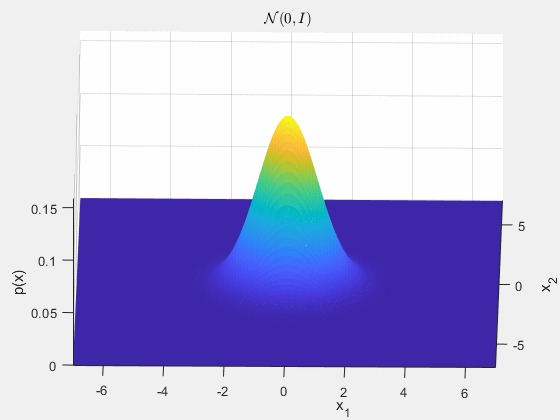
\includegraphics[width=8cm]{2d_gaussian.png}
    \caption{Probability density surface of a two-dimensional multivariate Gaussian distribution.}
    \label{fig:2d_gaussian}
\end{figure}


\subsection{State and Covariance Definitions}
The Kalman filter maintains the conditional mean and covariance of the state. We define:
- $\hat{x}_{k|k-1}$: The \textbf{a priori} state estimate at step $k$, given all measurements up to step $k-1$.
- $\hat{x}_{k|k}$: The \textbf{a posteriori} state estimate at step $k$, given all measurements up to step $k$.
- $P_{k|k-1}$: The \textbf{a priori} estimation error covariance matrix:
  \begin{equation}
P_{k|k-1} = \mathbb{E}\left[ (x_k - \hat{x}_{k|k-1})(x_k - \hat{x}_{k|k-1})^\trp \right] .
  \end{equation}
- $P_{k|k}$: The \textbf{a posteriori} estimation error covariance matrix:
  \begin{equation}
P_{k|k} = \mathbb{E}\left[ (x_k - \hat{x}_{k|k})(x_k - \hat{x}_{k|k})^\trp \right] .
  \end{equation}

The filter operates in two alternating phases: \textbf{Prediction (Time Update)} and \textbf{Correction (Measurement Update)}.

\subsection{Prediction Phase (Time Update)}
In the prediction phase, the filter projects the state and covariance ahead in time using the system dynamics.
\begin{enumerate}
    \item \textbf{State Prediction}:
    Since the noise $w_k$ is zero-mean and uncorrelated with previous states, the optimal prediction of the state is:
    \begin{equation}
        \hat{x}_{k|k-1} = A \hat{x}_{k-1|k-1} + B u_{k-1} , \label{eq:kf_pred_state}
    \end{equation}
    \item \textbf{Covariance Prediction}:
    Let us define the a priori error $e_{k|k-1} = x_k - \hat{x}_{k|k-1}$. Substituting the dynamics \eqref{eq:kf_state} and prediction \eqref{eq:kf_pred_state}:
    \begin{align}
        e_{k|k-1} &= (A x_{k-1} + B u_{k-1} + w_{k-1}) - (A \hat{x}_{k-1|k-1} + B u_{k-1}) \nonumber \\
&= A e_{k-1|k-1} + w_{k-1} .
    \end{align}
    The a priori covariance is:
    \begin{align}
        P_{k|k-1} &= \mathbb{E}[e_{k|k-1} e_{k|k-1}^\trp] \nonumber \\
        &= \mathbb{E}\left[ (A e_{k-1|k-1} + w_{k-1})(A e_{k-1|k-1} + w_{k-1})^\trp \right] \nonumber \\
&= A \mathbb{E}[e_{k-1|k-1} e_{k-1|k-1}^\trp] A^\trp + \mathbb{E}[w_{k-1} w_{k-1}^\trp] + A \mathbb{E}[e_{k-1|k-1} w_{k-1}^\trp] + \mathbb{E}[w_{k-1} e_{k-1|k-1}^\trp] A^\trp .
    \end{align}
    Since the process noise $w_{k-1}$ is white and uncorrelated with the past error $e_{k-1|k-1}$, the cross terms vanish. This simplifies to:
    \begin{equation}
        P_{k|k-1} = A P_{k-1|k-1} A^\trp + W . \label{eq:kf_pred_cov}
    \end{equation}
\end{enumerate}

\subsection{Correction Phase (Measurement Update)}
When a new measurement $y_k$ becomes available, we correct our prediction using a Luenberger-like update:
\begin{equation}
    \hat{x}_{k|k} = \hat{x}_{k|k-1} + K_k \left( y_k - C \hat{x}_{k|k-1} \right) , \label{eq:kf_corr_state}
\end{equation}
where $K_k \in \R^{n \times p}$ is the \textbf{Kalman Gain} to be determined.

To find the optimal gain $K_k$, we analyze the a posteriori error $e_{k|k} = x_k - \hat{x}_{k|k}$:
\begin{align}
    e_{k|k} &= x_k - \left( \hat{x}_{k|k-1} + K_k (C x_k + v_k - C \hat{x}_{k|k-1}) \right) \nonumber \\
&= (I - K_k C) e_{k|k-1} - K_k v_k .
\end{align}
The a posteriori covariance is:
\begin{align}
    P_{k|k} &= \mathbb{E}[e_{k|k} e_{k|k}^\trp] \nonumber \\
    &= \mathbb{E}\left[ \left( (I - K_k C) e_{k|k-1} - K_k v_k \right) \left( (I - K_k C) e_{k|k-1} - K_k v_k \right)^\trp \right] \nonumber \\
    &= (I - K_k C) \mathbb{E}[e_{k|k-1} e_{k|k-1}^\trp] (I - K_k C)^\trp + K_k \mathbb{E}[v_k v_k^\trp] K_k^\trp \nonumber \\
&\quad - (I - K_k C) \mathbb{E}[e_{k|k-1} v_k^\trp] K_k^\trp - K_k \mathbb{E}[v_k e_{k|k-1}^\trp] (I - K_k C)^\trp .
\end{align}
Since the sensor noise $v_k$ is uncorrelated with the a priori error $e_{k|k-1}$, the cross terms vanish:
\begin{equation}
    P_{k|k} = (I - K_k C) P_{k|k-1} (I - K_k C)^\trp + K_k V K_k^\trp . \label{eq:kf_joseph_form}
\end{equation}
Equation \eqref{eq:kf_joseph_form} is known as the \textbf{Joseph Form} of the covariance update, which is numerically stable and holds for any choice of gain $K_k$.

\subsection{Derivation of the Optimal Kalman Gain}
The optimal Kalman gain $K_k$ is defined as the gain that minimizes the total mean-squared estimation error, which is the sum of the variances of the state estimation errors. This is mathematically represented by the trace of the covariance matrix $P_{k|k}$:
\begin{equation}
\min_{K_k} \tr(P_{k|k}) .
\end{equation}
Expanding \eqref{eq:kf_joseph_form}:
\begin{equation}
P_{k|k} = P_{k|k-1} - K_k C P_{k|k-1} - P_{k|k-1} C^\trp K_k^\trp + K_k \left( C P_{k|k-1} C^\trp + V \right) K_k^\trp .
\end{equation}
Taking the trace of both sides and using the cyclic properties of the trace (e.g., $\tr(A) = \tr(A^\trp)$):
\begin{equation}
\tr(P_{k|k}) = \tr(P_{k|k-1}) - 2 \tr(K_k C P_{k|k-1}) + \tr\left( K_k (C P_{k|k-1} C^\trp + V) K_k^\trp \right) .
\end{equation}
To find the minimum, we take the matrix derivative with respect to $K_k$ and set it to zero:
\begin{equation}
\frac{\partial \tr(P_{k|k})}{\partial K_k} = -2 P_{k|k-1} C^\trp + 2 K_k \left( C P_{k|k-1} C^\trp + V \right) = 0 .
\end{equation}
Solving for $K_k$ yields the \textbf{optimal Kalman Gain}:
\begin{equation}
    K_k = P_{k|k-1} C^\trp \left( C P_{k|k-1} C^\trp + V \right)^{-1} . \label{eq:kf_optimal_gain}
\end{equation}

Substituting this optimal gain back into the Joseph form \eqref{eq:kf_joseph_form} simplifies the expression for the a posteriori covariance:
\begin{align}
    P_{k|k} &= (I - K_k C) P_{k|k-1} (I - K_k C)^\trp + K_k V K_k^\trp \nonumber \\
&= P_{k|k-1} - K_k C P_{k|k-1} - P_{k|k-1} C^\trp K_k^\trp + K_k (C P_{k|k-1} C^\trp + V) K_k^\trp .
\end{align}
Using $K_k (C P_{k|k-1} C^\trp + V) = P_{k|k-1} C^\trp$, the last two terms cancel:
\begin{equation}
    P_{k|k} = (I - K_k C) P_{k|k-1} . \label{eq:kf_corr_cov}
\end{equation}

\subsection{Summary of the Kalman Filter Algorithm}
The complete recursive equations of the Kalman filter are summarized in Table~\ref{tab:kalman_filter}.

\begin{table}[H]
\centering
\caption{The Discrete-Time Kalman Filter Algorithm}
\label{tab:kalman_filter}
\begin{tabular}{lll}
\toprule
\textbf{Phase} & \textbf{Equation} & \textbf{Description} \\
\midrule
\textbf{Prediction} & $\hat{x}_{k|k-1} = A \hat{x}_{k-1|k-1} + B u_{k-1}$ & Project the state ahead \\
                    & $P_{k|k-1} = A P_{k-1|k-1} A^\trp + W$ & Project the error covariance ahead \\
\midrule
\textbf{Correction} & $K_k = P_{k|k-1} C^\trp (C P_{k|k-1} C^\trp + V)^{-1}$ & Compute the optimal Kalman Gain \\
                    & $\hat{x}_{k|k} = \hat{x}_{k|k-1} + K_k (y_k - C \hat{x}_{k|k-1})$ & Update estimate with measurement \\
                    & $P_{k|k} = (I - K_k C) P_{k|k-1}$ & Update the error covariance \\
\bottomrule
\end{tabular}
\end{table}

Under the assumptions of stabilizability of $(A, B)$ and detectability of $(A, C)$, the error covariance converges to a steady-state value $P_{k|k-1} \to P$ as $k \to \infty$. This steady-state covariance satisfies the discrete Riccati equation:
\begin{equation}
P = A P A^\trp - A P C^\trp (C P C^\trp + V)^{-1} C P A^\top + W ,
\end{equation}
yielding a constant optimal filter gain $K = P C^\trp (C P C^\trp + V)^{-1}$. This steady-state estimator is identical in structure to a discrete Luenberger observer, but its gain is optimally tuned to balance process disturbances and sensor noise.

\section{Homework: State Observer for a Physical System}
\begin{figure}[H]
    \centering
    \includegraphics[width=5cm]{pendulum.png}
    \caption{State estimation task on an inverted pendulum system.}
    \label{fig:homework_observer_pendulum}
  \end{figure}
  
  \begin{exercise}
  Select a physical system of your interest (e.g., the inverted pendulum shown in Figure \ref{fig:homework_observer_pendulum}, a quadcopter, or a bioreactor). Design a Luenberger observer in continuous-time and verify that the observer poles are faster than the closed-loop controller poles. Under initial state mismatches, plot the estimated states alongside the actual states to demonstrate convergence of the estimation error.
  \end{exercise}

\chapter{Robust H2 Control via LMI}

\section{The H2 Norm of LTI Systems}
In modern control system design, we often need to evaluate how external disturbances affect system outputs. The $H_2$ norm is a fundamental performance metric that measures the "size" of a system's output response when subjected to impulsive inputs or white noise disturbances. Typical applications include minimizing control effort, regulating state deviations, and mitigating thermal noise in circuits.

Consider the stable, continuous-time LTI system:
\begin{align}
    \dot{x}(t) &= A x(t) + B_w w(t) \label{eq:h2_state} \\
    z(t) &= C_z x(t) + D_{zw} w(t) .\label{eq:h2_output}
\end{align}
where $x(t) \in \R^n$ is the state vector, $w(t) \in \R^m$ is the disturbance input vector, and $z(t) \in \R^r$ is the controlled output (or performance vector). 

For the $H_2$ norm to be finite, the transfer function matrix $G(s) = C_z (sI - A)^{-1} B_w + D_{zw}$ must be strictly proper, which requires:
\begin{equation}
D_{zw} = 0 .
\end{equation}
If $D_{zw} \neq 0$, the high-frequency gain of the system does not roll off to zero, and the system would pass high-frequency white noise with infinite energy, leading to an infinite $H_2$ norm. Thus, we restrict our attention to systems where $z(t) = C_z x(t)$.

\subsection{Frequency-Domain and Time-Domain Definitions}
In the frequency domain, the $H_2$ norm of the system $G(s) = C_z (sI - A)^{-1} B_w$ is defined as the root-mean-square of the frequency response over all frequencies:
\begin{equation}
    \| G \|_2 = \left( \frac{1}{2\pi} \int_{-\infty}^{\infty} \tr\left( G(j\omega) G(j\omega)^* \right) d\omega \right)^{1/2} .\label{eq:h2_freq}
\end{equation}
where $G(j\omega)^*$ is the conjugate transpose of $G(j\omega)$.

By Parseval's theorem, this frequency-domain definition is mathematically equivalent to the total energy of the system's impulse response in the time domain. Let $z^{(i)}(t)$ be the output response of the system starting from zero initial states when the $i$-th input is an impulse: $w(t) = \delta(t) e_i$, where $e_i$ is the $i$-th standard basis vector. The impulse response is:
\begin{equation}
z^{(i)}(t) = C_z e^{A t} B_w e_i .
\end{equation}
The squared $H_2$ norm is the sum of the $L_2$ norms of the output channels:
\begin{equation}
\| G \|_2^2 = \sum_{i=1}^m \int_0^\infty \| z^{(i)}(t) \|^2 dt = \int_0^\infty \tr\left( \left( C_z e^{A t} B_w \right)^\trp \left( C_z e^{A t} B_w \right) \right) dt .
\end{equation}
Using the cyclic property of the trace ($\tr(XY) = \tr(YX)$), we can write this in two dual ways:
\begin{align}
    \| G \|_2^2 &= \tr\left( B_w^\trp \left( \int_0^\infty e^{A^\trp t} C_z^\trp C_z e^{A t} dt \right) B_w \right) \label{eq:h2_obs_form} \\
    \| G \|_2^2 &= \tr\left( C_z \left( \int_0^\infty e^{A t} B_w B_w^\trp e^{A^\trp t} dt \right) C_z^\trp \right) .\label{eq:h2_cont_form}
\end{align}

We recognize the integrals inside the parentheses as the \textbf{Observability Gramian} $P_o$ and \textbf{Controllability Gramian} $P_c$, which satisfy the Lyapunov equations:
\begin{align}
    A^\trp P_o + P_o A + C_z^\trp C_z &= 0 \label{eq:h2_lyap_po} \\
    A P_c + P_c A^\trp + B_w B_w^\trp &= 0 .\label{eq:h2_lyap_pc}
\end{align}
Thus, the $H_2$ norm can be computed directly from these Gramians:
\begin{equation}
    \| G \|_2^2 = \tr(B_w^\trp P_o B_w) = \tr(C_z P_c C_z^\trp) .\label{eq:h2_gramian_val}
\end{equation}

\section{LMI Formulation of the H2 Norm}
To design controllers that optimize the $H_2$ norm under uncertainty, we represent the condition $\| G \|_2^2 < \gamma$ (where $\gamma > 0$ is a scalar performance bound) as a set of Linear Matrix Inequalities.

We utilize the controllability-based Gramian representation \eqref{eq:h2_cont_form}.

\begin{mytheorem}{LMI H2 Performance Condition}
The LTI system \eqref{eq:h2_state}--\eqref{eq:h2_output} (with $D_{zw}=0$) is asymptotically stable and satisfies $\| G \|_2^2 < \gamma$ if and only if there exist a symmetric positive definite matrix $W \in \R^{n \times n}$ and a symmetric matrix $Z \in \R^{r \times r}$ satisfying:
\begin{align}
    A W + W A^\trp + B_w B_w^\trp &\prec 0 \label{eq:h2_lmi_lyap} \\
    \begin{bmatrix} Z & C_z W \\ W C_z^\trp & W \end{bmatrix} &\succ 0 \label{eq:h2_lmi_schur} \\
    \tr(Z) &< \gamma .\label{eq:h2_lmi_trace}
\end{align}
\end{mytheorem}

\begin{proof}
Let $A$ be stable. The Lyapunov inequality \eqref{eq:h2_lmi_lyap} implies that the controllability Gramian $P_c$ satisfies:
\begin{equation}
P_c \prec W .
\end{equation}
Since $P_c \prec W$, we can bound the output covariance:
\begin{equation}
C_z P_c C_z^\trp \prec C_z W C_z^\trp .
\end{equation}
Taking the trace yields:
\begin{equation}
\| G \|_2^2 = \tr(C_z P_c C_z^\trp) < \tr(C_z W C_z^\trp) .
\end{equation}
Next, we apply the Schur complement to the block matrix inequality \eqref{eq:h2_lmi_schur}. The inequality is equivalent to:
\begin{equation}
W \succ 0 \quad \text{and} \quad Z - C_z W W^{-1} W C_z^\trp \succ 0 .
\end{equation}
This simplifies directly to:
\begin{equation}
Z \succ C_z W C_z^\trp .
\end{equation}
Taking the trace of this relation:
\begin{equation}
\tr(Z) > \tr(C_z W C_z^\trp) .
\end{equation}
Thus, if we enforce $\tr(Z) < \gamma$ in \eqref{eq:h2_lmi_trace}, we guarantee:
\begin{equation}
\| G \|_2^2 < \tr(C_z W C_z^\trp) < \tr(Z) < \gamma .
\end{equation}
which proves the theorem.
\end{proof}

\section{H2 State Feedback Controller Design}
We now apply this LMI formulation to design an optimal robust state feedback controller. Consider the system:
\begin{align}
    \dot{x}(t) &= A x(t) + B_u u(t) + B_w w(t) \\
z(t) &= C_z x(t) + D_{zu} u(t) .
\end{align}
where $u(t)$ is the control input. We wish to design a state feedback gain $K \in \R^{m \times n}$ such that the control law:
\begin{equation}
u(t) = -K x(t) .
\end{equation}
stabilizes the closed-loop system and minimizes the $H_2$ norm of the closed-loop transfer function $G_{cl}(s)$ from $w$ to $z$.

The closed-loop dynamics are:
\begin{align}
    \dot{x}(t) &= (A - B_u K) x(t) + B_w w(t) \\
z(t) &= (C_z - D_{zu} K) x(t) .
\end{align}
Applying the $H_2$ LMI theorem, the closed-loop system is stable and satisfies $\| G_{cl} \|_2^2 < \gamma$ if there exist $W \succ 0$ and $Z = Z^\trp$ such that:
\begin{align}
    (A - B_u K) W + W (A - B_u K)^\trp + B_w B_w^\trp &\prec 0 \label{eq:h2_bmi_1} \\
    \begin{bmatrix} Z & (C_z - D_{zu} K) W \\ W (C_z - D_{zu} K)^\trp & W \end{bmatrix} &\succ 0 \label{eq:h2_bmi_2} \\
\tr(Z) &< \gamma .
\end{align}
These inequalities are Bilinear Matrix Inequalities because of the products $KW$ in both expressions.

To linearize the system, we introduce the auxiliary variable:
\begin{equation}
Y = K W \in \R^{m \times n} \implies Y^\trp = W K^\trp .
\end{equation}
Substituting $Y$ and $Y^\trp$ into \eqref{eq:h2_bmi_1} and \eqref{eq:h2_bmi_2} gives:
\begin{align}
    (A - B_u K) W + W (A - B_u K)^\trp &= A W - B_u (KW) + W A^\trp - (W K^\trp) B_u^\trp \nonumber \\
&= A W + W A^\trp - B_u Y - Y^\trp B_u^\trp .
\end{align}
and:
\begin{equation}
(C_z - D_{zu} K) W = C_z W - D_{zu} Y .
\end{equation}

This leads directly to the $H_2$ state-feedback synthesis theorem.

\begin{mytheorem}{H2 State Feedback LMI Synthesis}
The optimal $H_2$ state feedback design problem is solved by the following convex semidefinite program:
\begin{equation}
\min_{W, Y, Z} \gamma \quad \text{subject to} .
\end{equation}
\begin{align}
    W &\succ 0 \\
    A W + W A^\trp - B_u Y - Y^\trp B_u^\trp + B_w B_w^\trp &\prec 0 \label{eq:h2_sf_lmi1} \\
    \begin{bmatrix} Z & C_z W - D_{zu} Y \\ W C_z^\trp - Y^\trp D_{zu}^\trp & W \end{bmatrix} &\succ 0 \label{eq:h2_sf_lmi2} \\
\tr(Z) &< \gamma .
\end{align}
The optimal robust feedback gain is reconstructed as:
\begin{equation}
K^* = Y^* (W^*)^{-1} .
\end{equation}
\end{mytheorem}

This LMI formulation is extremely powerful. If the matrices $A$ and $B_u$ belong to a polytopic uncertainty set, we can robustly guarantee $\| G_{cl} \|_2^2 < \gamma$ for the entire polytope by solving \eqref{eq:h2_sf_lmi1} and \eqref{eq:h2_sf_lmi2} simultaneously at each vertex using the single, common decision variables $W$, $Y$, and $Z$!

\chapter{Robust H-infinity Control}

\section{The H-infinity Norm of LTI Systems}
In practical engineering systems, mathematical models are never perfect. Parameter variations, unmodeled high-frequency dynamics, and physical wear introduce unstructured perturbations. The $H_\infty$ norm is the key mathematical tool in robust control theory used to quantify a system's worst-case performance and guarantee robust stability in the presence of these model uncertainties.

Consider the stable, continuous-time LTI system:
\begin{align}
    \dot{x}(t) &= A x(t) + B_w w(t) \label{eq:hinf_state} \\
    z(t) &= C_z x(t) + D_{zw} w(t) , \label{eq:hinf_output}
\end{align}
where $w(t) \in \R^m$ represents worst-case external disturbances, and $z(t) \in \R^r$ is the controlled output performance vector.

\subsection{Frequency-Domain and Time-Domain Definitions}
In the frequency domain, the $H_\infty$ norm of the transfer function $G(s) = C_z (sI - A)^{-1} B_w + D_{zw}$ is defined as the peak gain (or maximum singular value) of the system over all frequencies:
\begin{equation}
    \| G \|_\infty = \sup_{\omega \in \R} \sigma_{\max}\left( G(j\omega) \right) , \label{eq:hinf_freq}
\end{equation}
where $\sigma_{\max}(\cdot)$ denotes the maximum singular value of the matrix.

\begin{figure}[H]
    \centering
    \includegraphics[width=9.5cm]{hinf_norm.png}
    \caption{H-infinity norm defined as the peak singular value over all frequencies.}
    \label{fig:hinf_norm}
\end{figure}

In the time domain, the $H_\infty$ norm corresponds to the \textbf{induced $L_2$-to-$L_2$ norm} of the system. Let $L_2$ be the space of square-integrable signals:
\begin{equation}
\| w \|_{L_2} = \left( \int_0^\infty \| w(t) \|^2 dt \right)^{1/2} < \infty .
\end{equation}
Assuming zero initial conditions ($x(0) = 0$), the $H_\infty$ norm is defined as:
\begin{equation}
    \| G \|_\infty = \sup_{w \neq 0, w \in L_2} \frac{\| z \|_{L_2}}{\| w \|_{L_2}} = \sup_{w \neq 0, w \in L_2} \frac{\left( \int_0^\infty \| z(t) \|^2 dt \right)^{1/2}}{\left( \int_0^\infty \| w(t) \|^2 dt \right)^{1/2}} . \label{eq:hinf_time}
\end{equation}
This indicates the worst-case disturbance amplification ratio. For any disturbance signal $w(t)$, the output energy is guaranteed to satisfy:
\begin{equation}
\| z \|_{L_2} \le \| G \|_\infty \| w \|_{L_2} .
\end{equation}

\section{The Bounded Real Lemma (BRL)}
Evaluating the $H_\infty$ norm using the frequency-domain definition \eqref{eq:hinf_freq} requires sweeping across all frequencies, which is computationally cumbersome. The \textbf{Bounded Real Lemma (BRL)} provides a state-space characterization of the $H_\infty$ norm, formulating the inequality $\| G \|_\infty < \gamma$ as a single Linear Matrix Inequality.

\begin{mytheorem}{Continuous-Time Bounded Real Lemma}
The LTI system \eqref{eq:hinf_state}--\eqref{eq:hinf_output} is asymptotically stable and satisfies $\| G \|_\infty < \gamma$ if and only if there exists a symmetric positive definite matrix $P \in \R^{n \times n}$ satisfying:
\begin{equation}
    \begin{bmatrix} A^\trp P + P A & P B_w & C_z^\trp \\ B_w^\trp P & -\gamma I & D_{zw}^\trp \\ C_z & D_{zw} & -\gamma I \end{bmatrix} \prec 0 . \label{eq:brl_lmi}
\end{equation}
\end{mytheorem}

\begin{proof}
We prove the sufficiency ($\Leftarrow$) of the BRL. Assume there exists $P \succ 0$ satisfying the LMI \eqref{eq:brl_lmi}. We define a quadratic Lyapunov (or storage) function:
\begin{equation}
V(x(t)) = x(t)^\trp P x(t) \ge 0 .
\end{equation}
Differentiating $V(x(t))$ along the system trajectories $\dot{x} = A x + B_w w$ yields:
\begin{align}
    \dot{V}(x) &= \dot{x}^\trp P x + x^\trp P \dot{x} \nonumber \\
    &= (A x + B_w w)^\trp P x + x^\trp P (A x + B_w w) \nonumber \\
    &= x^\trp (A^\trp P + P A) x + 2 x^\trp P B_w w . \label{eq:brl_vdot}
\end{align}
To establish $\| G \|_\infty < \gamma$, we seek to show that for any non-zero disturbance $w(t) \in L_2$ under $x(0) = 0$, we have:
\begin{equation}
\| z \|_{L_2}^2 < \gamma^2 \| w \|_{L_2}^2 \implies \int_0^\infty \left( \| z(t) \|^2 - \gamma^2 \| w(t) \|^2 \right) dt < 0 .
\end{equation}
Let us define the Hamiltonian-like dissipation term:
\begin{equation}
    \mathcal{D}(x, w) = \dot{V}(x) + \frac{1}{\gamma} \| z(t) \|^2 - \gamma \| w(t) \|^2 . \label{eq:brl_dissipation}
\end{equation}
Substitute $z(t) = C_z x(t) + D_{zw} w(t)$ and $\dot{V}(x)$ from \eqref{eq:brl_vdot} into \eqref{eq:brl_dissipation}:
\begin{align}
    \mathcal{D}(x, w) &= x^\trp (A^\trp P + P A) x + 2 x^\trp P B_w w \nonumber \\
&\quad + \frac{1}{\gamma} (C_z x + D_{zw} w)^\trp (C_z x + D_{zw} w) - \gamma w^\trp w .
\end{align}
We can write this quadratic form compactly as:
\begin{equation}
\mathcal{D}(x, w) = \begin{bmatrix} x \\ w \end{bmatrix}^\trp \begin{bmatrix} A^\trp P + P A + \frac{1}{\gamma} C_z^\trp C_z & P B_w + \frac{1}{\gamma} C_z^\trp D_{zw} \\ B_w^\trp P + \frac{1}{\gamma} D_{zw}^\trp C_z & \frac{1}{\gamma} D_{zw}^\trp D_{zw} - \gamma I \end{bmatrix} \begin{bmatrix} x \\ w \end{bmatrix} .
\end{equation}
For the system to satisfy the dissipation inequality $\mathcal{D}(x, w) < 0$ for all $\begin{bmatrix} x^\trp & w^\trp \end{bmatrix}^\trp \neq 0$, the central matrix must be strictly negative definite:
\begin{equation}
    \begin{bmatrix} A^\trp P + P A + \frac{1}{\gamma} C_z^\trp C_z & P B_w + \frac{1}{\gamma} C_z^\trp D_{zw} \\ B_w^\trp P + \frac{1}{\gamma} D_{zw}^\trp C_z & \frac{1}{\gamma} D_{zw}^\trp D_{zw} - \gamma I \end{bmatrix} \prec 0 . \label{eq:brl_proof_schur_pre}
\end{equation}
We can rewrite this matrix by separating the terms involving $C_z$ and $D_{zw}$:
\begin{equation}
\begin{bmatrix} A^\trp P + P A & P B_w \\ B_w^\trp P & -\gamma I \end{bmatrix} + \frac{1}{\gamma} \begin{bmatrix} C_z^\trp \\ D_{zw}^\trp \end{bmatrix} \begin{bmatrix} C_z & D_{zw} \end{bmatrix} \prec 0 .
\end{equation}
Applying the Schur complement to this expression immediately yields the BRL LMI:
\begin{equation}
\begin{bmatrix} A^\trp P + P A & P B_w & C_z^\trp \\ B_w^\trp P & -\gamma I & D_{zw}^\trp \\ C_z & D_{zw} & -\gamma I \end{bmatrix} \prec 0 .
\end{equation}
Now, integrating $\mathcal{D}(x, w) < 0$ from $t = 0$ to $t = \infty$:
\begin{equation}
\int_0^\infty \dot{V}(x(t)) dt + \frac{1}{\gamma} \int_0^\infty \| z(t) \|^2 dt - \gamma \int_0^\infty \| w(t) \|^2 dt < 0 .
\end{equation}
Since $x(0) = 0$ and the system is stable ($\lim_{t\to\infty} x(t) = 0$), the first term evaluates to:
\begin{equation}
\int_0^\infty \dot{V}(x(t)) dt = V(x(\infty)) - V(x(0)) = 0 .
\end{equation}
Thus, we have:
\begin{equation}
\frac{1}{\gamma} \| z \|_{L_2}^2 - \gamma \| w \|_{L_2}^2 < 0 \implies \| z \|_{L_2}^2 < \gamma^2 \| w \|_{L_2}^2 .
\end{equation}
This completes the proof of sufficiency.
\end{proof}

\subsection{Discrete-Time Bounded Real Lemma}
For discrete-time systems $x_{k+1} = A x_k + B w_k$, $z_k = C_z x_k + D_{zw} w_k$, the discrete-time BRL characterizes the performance $\| G \|_\infty < \gamma$ using the following LMI.

\begin{mytheorem}{Discrete-Time Bounded Real Lemma}
The discrete LTI system is asymptotically stable and satisfies $\| G \|_\infty < \gamma$ if and only if there exists a symmetric positive definite matrix $P \in \R^{n \times n}$ satisfying:
\begin{equation}
    \begin{bmatrix} A^\trp P A - P & A^\trp P B_w & C_z^\trp \\ B_w^\trp P A & B_w^\trp P B_w - \gamma I & D_{zw}^\trp \\ C_z & D_{zw} & -\gamma I \end{bmatrix} \prec 0 . \label{eq:brl_dt_lmi}
\end{equation}
\end{mytheorem}

\begin{figure}[H]
    \centering
    \includegraphics[width=9.5cm]{hinf_norm_discrete.png}
    \caption{Discrete-time H-infinity norm maximum singular value frequency plot.}
    \label{fig:hinf_norm_discrete}
\end{figure}

\section{Robust H-infinity State Feedback Synthesis}
We now design a state feedback gain $K \in \R^{m \times n}$ for the system:
\begin{align}
    \dot{x}(t) &= A x(t) + B_u u(t) + B_w w(t) \\
z(t) &= C_z x(t) + D_{zu} u(t) ,
\end{align}
such that the closed-loop system under the control law $u(t) = -K x(t)$ is stable and satisfies $\| G_{cl} \|_\infty < \gamma$. We assume $D_{zw} = 0$ to focus on the essential LMI structure.

The closed-loop dynamics are:
\begin{align}
    \dot{x}(t) &= (A - B_u K) x(t) + B_w w(t) \\
z(t) &= (C_z - D_{zu} K) x(t) .
\end{align}
Applying the continuous-time BRL \eqref{eq:brl_lmi} with $D_{zw} = 0$, the closed loop satisfies $\| G_{cl} \|_\infty < \gamma$ if there exists $P \succ 0$ satisfying:
\begin{equation}
    \begin{bmatrix} (A - B_u K)^\trp P + P (A - B_u K) & P B_w & (C_z - D_{zu} K)^\trp \\ B_w^\trp P & -\gamma I & 0 \\ C_z - D_{zu} K & 0 & -\gamma I \end{bmatrix} \prec 0 . \label{eq:hinf_bmi}
\end{equation}
This is a BMI due to the products of the decision variables $P$ and $K$.

To linearize the inequality, we perform a congruence transformation:
\begin{enumerate}
    \item Define $W = P^{-1} \succ 0$.
    \item Pre- and post-multiply \eqref{eq:hinf_bmi} by the block diagonal matrix $\text{diag}(W, I, I)$:
    \begin{equation}
\begin{bmatrix} W & 0 & 0 \\ 0 & I & 0 \\ 0 & 0 & I \end{bmatrix} \begin{bmatrix} (A - B_u K)^\trp P + P (A - B_u K) & P B_w & (C_z - D_{zu} K)^\trp \\ B_w^\trp P & -\gamma I & 0 \\ C_z - D_{zu} K & 0 & -\gamma I \end{bmatrix} \begin{bmatrix} W & 0 & 0 \\ 0 & I & 0 \\ 0 & 0 & I \end{bmatrix} \prec 0 .
    \end{equation}
    This simplifies to:
    \begin{equation}
\begin{bmatrix} W (A - B_u K)^\trp + (A - B_u K) W & B_w & W (C_z - D_{zu} K)^\trp \\ B_w^\trp & -\gamma I & 0 \\ (C_z - D_{zu} K) W & 0 & -\gamma I \end{bmatrix} \prec 0 .
    \end{equation}
    \item Define the auxiliary variable $Y = K W$, which yields:
    \begin{equation}
\begin{bmatrix} A W + W A^\trp - B_u Y - Y^\trp B_u^\trp & B_w & W C_z^\trp - Y^\trp D_{zu}^\trp \\ B_w^\trp & -\gamma I & 0 \\ C_z W - D_{zu} Y & 0 & -\gamma I \end{bmatrix} \prec 0 .
    \end{equation}
\end{enumerate}

This leads directly to the robust $H_\infty$ synthesis theorem.

\begin{mytheorem}{H-infinity State Feedback LMI Synthesis}
The robust $H_\infty$ state feedback gain $K$ that minimizes the worst-case disturbance amplification $\gamma$ is solved by the following convex semidefinite program:
\begin{equation}
\min_{W, Y} \gamma \quad \text{subject to} .
\end{equation}
\begin{align}
    W &\succ 0 \\
    \begin{bmatrix} A W + W A^\trp - B_u Y - Y^\trp B_u^\trp & B_w & W C_z^\trp - Y^\trp D_{zu}^\trp \\ B_w^\trp & -\gamma I & 0 \\ C_z W - D_{zu} Y & 0 & -\gamma I \end{bmatrix} &\prec 0 . \label{eq:hinf_sf_lmi}
\end{align}
The optimal feedback gain is reconstructed as:
\begin{equation}
K^* = Y^* (W^*)^{-1} .
\end{equation}
\end{mytheorem}
If the system matrices $[A \quad B_u]$ are subject to polytopic uncertainty, we can solve the LMI \eqref{eq:hinf_sf_lmi} simultaneously at all vertices using the single common variables $W$ and $Y$. This guarantees robust stability and a guaranteed $H_\infty$ attenuation bound $\gamma$ for all plants in the uncertainty polytope.

\chapter{Robust H2/Hinf Filtering}

\section{The Robust State Estimation and Filtering Problem}
In previous chapters, we designed state observers under the assumption of perfect plant models and known noise statistics. However, in real-world systems, the plant parameters (e.g., mass, stiffness, resistance) are subject to variations, and the spectral densities of the environmental noise are rarely known with precision.

Under such conditions, a standard Kalman filter can lose its optimality or even diverge. To address this, **robust filtering** designs estimators that guarantee a bound on the estimation error energy, regardless of parameter variations and the exact nature of the noise, by utilizing $H_2$ and $H_\infty$ performance bounds.

Consider the continuous-time LTI system under parameter uncertainty:
\begin{align}
    \dot{x}(t) &= A x(t) + B_w w(t) \label{eq:filt_plant_state} \\
    y(t) &= C_y x(t) + D_{yw} w(t) \label{eq:filt_plant_output} \\
    z(t) &= C_z x(t) \label{eq:filt_signal_to_est}
\end{align}
where $w(t) \in \R^m$ represents external noise and disturbances (which may include process and measurement noises), $y(t) \in \R^p$ is the vector of measured outputs, and $z(t) \in \R^r$ is the specific linear combination of states we wish to estimate.

We design a full-order linear filter (estimator) that has the structure of a Luenberger observer:
\begin{align}
    \dot{\hat{x}}(t) &= A \hat{x}(t) + L \left( y(t) - C_y \hat{x}(t) \right) \label{eq:filt_observer} \\
    \hat{z}(t) &= C_z \hat{x}(t) \label{eq:filt_est_output}
\end{align}
where $L \in \R^{n \times p}$ is the filter gain matrix to be designed.

\subsection{Estimation Error Dynamics}
Let us define the state estimation error $e_x(t) = x(t) - \hat{x}(t)$ and the signal estimation error $e_z(t) = z(t) - \hat{z}(t)$. Differentiating the state error yields:
\begin{align}
    \dot{e}_x(t) &= \dot{x}(t) - \dot{\hat{x}}(t) \nonumber \\
    &= (A x + B_w w) - \left( A \hat{x} + L (C_y x + D_{yw} w - C_y \hat{x}) \right) \nonumber \\
    &= (A - L C_y) (x - \hat{x}) + (B_w - L D_{yw}) w \nonumber \\
    &= (A - L C_y) e_x(t) + (B_w - L D_{yw}) w(t) \label{eq:filt_error_dynamics}
\end{align}
The signal estimation error is:
\begin{equation}
    e_z(t) = C_z x(t) - C_z \hat{x}(t) = C_z e_x(t) \label{eq:filt_output_error}
\end{equation}

Thus, the error system $G_{ew}(s)$ from the disturbance $w$ to the estimation error $e_z$ is governed by the state-space equations:
\begin{align}
    \dot{e}_x(t) &= A_{cl,f} e_x(t) + B_{cl,f} w(t) \\
    e_z(t) &= C_{cl,f} e_x(t)
\end{align}
where the closed-loop filter matrices are:
\begin{equation}
    A_{cl,f} = A - L C_y, \quad B_{cl,f} = B_w - L D_{yw}, \quad C_{cl,f} = C_z
\end{equation}

\section{Robust H-infinity Filter Design via LMI}
We first consider the $H_\infty$ performance criterion, which minimizes the worst-case disturbance amplification from the noise $w$ to the estimation error $e_z$:
\begin{equation}
    \| G_{ew} \|_\infty = \sup_{w \neq 0, w \in L_2} \frac{\| e_z \|_{L_2}}{\| w \|_{L_2}} < \gamma_f
\end{equation}

Applying the Bounded Real Lemma (Theorem 8.2) to the error system, the filter error dynamics are asymptotically stable and $\| G_{ew} \|_\infty < \gamma_f$ if and only if there exists a symmetric positive definite matrix $P \in \R^{n \times n}$ such that:
\begin{equation}
    \begin{bmatrix} (A - L C_y)^\trp P + P (A - L C_y) & P (B_w - L D_{yw}) & C_z^\trp \\ (B_w - L D_{yw})^\trp P & -\gamma_f I & 0 \\ C_z & 0 & -\gamma_f I \end{bmatrix} \prec 0 \label{eq:filt_hinf_bmi}
\end{equation}
This inequality is a Bilinear Matrix Inequality because of the terms $P L C_y$ and $P L D_{yw}$.

\subsection{Linearization of the H-infinity Filtering BMI}
In the state feedback design, we linearized the BMI by defining $W = P^{-1}$ and pre- and post-multiplying by $W$. In the filtering design, this congruence transformation does not work because the observer gain $L$ is multiplied by $P$ from the left.

Instead, we perform a different, highly elegant linearization: we directly define a new decision variable:
\begin{equation}
    F = P L \in \R^{n \times p} \label{eq:filt_change_var}
\end{equation}
Since $P \succ 0$ is positive definite, it is invertible. Once $P$ and $F$ are found, we can reconstruct the filter gain uniquely as:
\begin{equation}
    L = P^{-1} F \label{eq:filt_reconstruct_gain}
\end{equation}

Substituting $F = P L$ into the terms of \eqref{eq:filt_hinf_bmi}:
\begin{align}
    P (A - L C_y) &= P A - (PL) C_y = P A - F C_y \\
    P (B_w - L D_{yw}) &= P B_w - (PL) D_{yw} = P B_w - F D_{yw}
\end{align}
The transposed terms are:
\begin{align}
    (A - L C_y)^\trp P &= A^\trp P - C_y^\trp F^\trp \\
    (B_w - L D_{yw})^\trp P &= B_w^\trp P - D_{yw}^\trp F^\trp
\end{align}

Substituting these expressions directly into \eqref{eq:filt_hinf_bmi} yields a standard convex LMI.

\begin{mytheorem}{Robust H-infinity Filter LMI Synthesis}
The robust $H_\infty$ filtering design problem is solved by the following convex semidefinite program:
\begin{equation}
    \min_{P, F} \gamma_f \quad \text{subject to}
\end{equation}
\begin{align}
    P &\succ 0 \\
    \begin{bmatrix} A^\trp P + P A - C_y^\trp F^\trp - F C_y & P B_w - F D_{yw} & C_z^\trp \\ B_w^\trp P - D_{yw}^\trp F^\trp & -\gamma_f I & 0 \\ C_z & 0 & -\gamma_f I \end{bmatrix} &\prec 0 \label{eq:filt_hinf_lmi}
\end{align}
The optimal robust filter gain is reconstructed as:
\begin{equation}
    L^* = (P^*)^{-1} F^*
\end{equation}
\end{mytheorem}

\section{Robust H2 Filter Design via LMI}
We now consider the $H_2$ performance criterion, which minimizes the estimation error energy when the system is driven by white Gaussian noise:
\begin{equation}
    \| G_{ew} \|_2^2 < \gamma_2
\end{equation}
Using the observability-based Gramian characterization of the $H_2$ norm, the error system is asymptotically stable and satisfies $\| G_{ew} \|_2^2 < \gamma_2$ if there exist $P \succ 0$ and a symmetric matrix $Z \in \R^{m \times m}$ such that:
\begin{align}
    \begin{bmatrix} (A - L C_y)^\trp P + P (A - L C_y) & C_z^\trp \\ C_z & -I \end{bmatrix} &\prec 0 \label{eq:filt_h2_bmi_1} \\
    \begin{bmatrix} Z & (B_w - L D_{yw})^\trp P \\ P (B_w - L D_{yw}) & P \end{bmatrix} &\succ 0 \label{eq:filt_h2_bmi_2} \\
    \tr(Z) &< \gamma_2
\end{align}

Using the exact same change of variables $F = P L$, these inequalities become convex LMIs.

\begin{mytheorem}{Robust H2 Filter LMI Synthesis}
The robust $H_2$ filtering design problem is solved by the following convex semidefinite program:
\begin{equation}
    \min_{P, F, Z} \gamma_2 \quad \text{subject to}
\end{equation}
\begin{align}
    P &\succ 0 \\
    \begin{bmatrix} A^\trp P + P A - C_y^\trp F^\trp - F C_y & C_z^\trp \\ C_z & -I \end{bmatrix} &\prec 0 \label{eq:filt_h2_lmi1} \\
    \begin{bmatrix} Z & B_w^\trp P - D_{yw}^\trp F^\trp \\ P B_w - F D_{yw} & P \end{bmatrix} &\succ 0 \label{eq:filt_h2_lmi2} \\
    \tr(Z) &< \gamma_2
\end{align}
The optimal robust $H_2$ filter gain is reconstructed as:
\begin{equation}
    L^* = (P^*)^{-1} F^*
\end{equation}
\end{mytheorem}

\subsection{Multiobjective H2/Hinf Filtering}
In many practical scenarios, we want to balance the worst-case disturbance rejection ($H_\infty$) and average-case white noise regulation ($H_2$). This is known as **multiobjective filtering**. Because both problems share the exact same optimization variable $P$ and change of variables $F = P L$, we can solve them simultaneously with a single shared Lyapunov matrix $P$, yielding a filter gain $L = P^{-1}F$ that satisfies both criteria:
\begin{equation}
    \min_{P, F, Z} \alpha \gamma_f + (1-\alpha) \gamma_2 \quad \text{subject to } \text{\eqref{eq:filt_hinf_lmi}, \eqref{eq:filt_h2_lmi1}, \eqref{eq:filt_h2_lmi2}}
\end{equation}
where $\alpha \in [0, 1]$ is a relative weighting factor chosen by the designer. This highlights the immense power and flexibility of the LMI framework in modern graduate-level control theory.

\chapter{Robust Control of Sampled-Data Systems via DLMI}

\section{Introduction to Sampled-Data Systems}
Physical systems (such as aircraft, chemical reactors, and electrical grids) are continuous-time dynamical processes governed by differential equations. However, modern controllers are implemented on digital computers, microcontrollers, or distributed networks. The coupling of a continuous plant with a discrete digital controller results in a **sampled-data system**, which is hybrid in nature.

Consider the continuous-time LTI plant dynamics:
\begin{equation}
    \dot{x}(t) = A x(t) + B u(t) \label{eq:sd_plant}
\end{equation}
A digital controller samples the state vector $x(t)$ at discrete time instants $t_k$, computes the control input vector $u_k = -K x(t_k)$ using a state feedback gain $K$, and holds this control signal constant between sampling instants using a **Zero-Order Hold (ZOH)**:
\begin{equation}
    u(t) = u_k = -K x(t_k) \quad \text{for } t \in [t_k, t_{k+1}) \label{eq:sd_zoh}
\end{equation}
Substituting \eqref{eq:sd_zoh} into \eqref{eq:sd_plant} yields the hybrid closed-loop system:
\begin{equation}
    \dot{x}(t) = A x(t) - B K x(t_k) \quad \text{for } t \in [t_k, t_{k+1}) \label{eq:sd_cl}
\end{equation}
The sampling interval is denoted by $h_k = t_{k+1} - t_k > 0$. In general, the sampling intervals can be time-varying due to digital network delays, packet drops, or OS scheduling jitter:
\begin{equation}
    h_k \in [h_{\min}, h_{\max}]
\end{equation}
The presence of the term $x(t_k)$ makes the closed-loop system time-varying and infinite-dimensional, rendering standard continuous Lyapunov stability analysis ($A_{cl}^\trp P + P A_{cl} \prec 0$) inapplicable.

\section{Lyapunov Stability Analysis via Looped Functionals}
To analyze stability under variable sampling intervals, a standard quadratic Lyapunov function candidate $V(x(t)) = x(t)^\trp P x(t)$ with a constant $P \succ 0$ is highly conservative. It would require the energy to decrease monotonically at *every* continuous time instant $t$, which is unnecessary. We only require the energy to decrease from one sampling instant to the next, i.e., $V(x(t_{k+1})) < V(x(t_k))$.

To achieve this, we employ the **Looped Lyapunov Functional** approach.

Let us define a functional of the form:
\begin{equation}
    V(t) = x(t)^\trp P x(t) + \mathcal{V}_0(t), \quad t \in [t_k, t_{k+1}) \label{eq:sd_looped_lyap}
\end{equation}
where $\mathcal{V}_0(t)$ is a time-dependent looped term satisfying the boundary conditions:
\begin{equation}
    \mathcal{V}_0(t_k) = \mathcal{V}_0(t_{k+1}) = 0 \label{eq:sd_boundary}
\end{equation}
Because of the boundary conditions \eqref{eq:sd_boundary}, evaluating \eqref{eq:sd_looped_lyap} at the sampling instants yields:
\begin{equation}
    V(t_k) = x(t_k)^\trp P x(t_k) \quad \text{and} \quad V(t_{k+1}) = x(t_{k+1})^\trp P x(t_{k+1})
\end{equation}
If we can guarantee that the derivative of the functional is strictly negative throughout the sampling interval:
\begin{equation}
    \dot{V}(t) = \frac{d}{dt} \left( x(t)^\trp P x(t) + \mathcal{V}_0(t) \right) < 0 \quad \text{for all } t \in [t_k, t_{k+1})
\end{equation}
then integrating this derivative from $t_k$ to $t_{k+1}$ guarantees:
\begin{equation}
    V(t_{k+1}) - V(t_k) = x(t_{k+1})^\trp P x(t_{k+1}) - x(t_k)^\trp P x(t_k) < 0
\end{equation}
This establishes asymptotic stability at the sampling instants, which implies continuous-time stability because the states cannot escape (blow up) within a finite sampling interval.

\section{Differential LMI (DLMI) Formulation}
A powerful way to represent the looped Lyapunov functional is to allow the Lyapunov matrix to be time-varying within each sampling interval. Let $\tau(t) = t - t_k \in [0, h_k]$ represent the elapsed time since the last sample. We propose a time-dependent Lyapunov candidate:
\begin{equation}
    V(x(t), \tau(t)) = x(t)^\trp P(\tau) x(t)
\end{equation}
where $P(\tau) = P(\tau)^\trp \succ 0$ is a continuously differentiable matrix function satisfying the boundary conditions:
\begin{equation}
    P(0) = P(h_k) = P_0 \succ 0
\end{equation}
Differentiating $V(x(t), \tau(t))$ along the trajectories of \eqref{eq:sd_cl} gives:
\begin{equation}
    \dot{V}(t) = \dot{x}(t)^\trp P(\tau) x(t) + x(t)^\trp P(\tau) \dot{x}(t) + x(t)^\trp \dot{P}(\tau) x(t)
\end{equation}
where $\dot{P}(\tau) = \frac{dP(\tau)}{d\tau}$.

Substituting the dynamics $\dot{x}(t) = A x(t) - B K x(t_k)$ and defining the augmented state vector $\eta(t) = \begin{bmatrix} x(t)^\trp & x(t_k)^\trp \end{bmatrix}^\trp$, we can write $\dot{V}(t)$ as:
\begin{equation}
    \dot{V}(t) = \eta(t)^\trp \begin{bmatrix} A^\trp P(\tau) + P(\tau) A + \dot{P}(\tau) & -P(\tau) B K \\ -K^\trp B^\trp P(\tau) & 0 \end{bmatrix} \eta(t)
\end{equation}
For stability, we require this quadratic form to be negative definite, which yields the **Differential Linear Matrix Inequality (DLMI)**:
\begin{equation}
    \begin{bmatrix} A^\trp P(\tau) + P(\tau) A + \dot{P}(\tau) & -P(\tau) B K \\ -K^\trp B^\trp P(\tau) & 0 \end{bmatrix} \prec 0, \quad \forall \tau \in [0, h_k] \label{eq:sd_dlmi}
\end{equation}

\section{Numerical Solution via Multi-Vertex Parameterization}
Directly solving the DLMI \eqref{eq:sd_dlmi} is challenging because it must hold for infinitely many points $\tau \in [0, h_k]$, and it is nonlinear due to the product $P(\tau)BK$.

To render it solvable, we parameterize $P(\tau)$ as an affine function of $\tau$:
\begin{equation}
    P(\tau) = \left( 1 - \frac{\tau}{h_k} \right) P_1 + \frac{\tau}{h_k} P_2 \label{eq:sd_p_param}
\end{equation}
where $P_1 \succ 0$ and $P_2 \succ 0$ are symmetric positive definite matrices.

Taking the derivative of \eqref{eq:sd_p_param} with respect to $\tau$ yields a constant matrix:
\begin{equation}
    \dot{P}(\tau) = \frac{P_2 - P_1}{h_k}
\end{equation}
Because the DLMI is affine in $\tau$, it is guaranteed to hold for all $\tau \in [0, h_k]$ if and only if it holds at the boundary vertices $\tau = 0$ and $\tau = h_k$. This reduces the infinite-dimensional DLMI to a finite set of LMIs.

To linearize the terms involving the controller gain $K$, we perform a congruence transformation:
\begin{enumerate}
    \item Define the inverse matrices $W(\tau) = P(\tau)^{-1}$.
    \item Pre- and post-multiply the DLMI \eqref{eq:sd_dlmi} by $\text{diag}(W(\tau), W(\tau))$.
    \item Define $Y = K W_0$ where $W_0 = P_0^{-1}$.
\end{enumerate}
This yields a set of standard, convex LMIs evaluated at the vertices.

\begin{mytheorem}{Robust Sampled-Data State Feedback DLMI Synthesis}
The sampled-data hybrid system \eqref{eq:sd_cl} is stable for any variable sampling interval $h_k \in [0, h]$ if there exist symmetric matrices $W_1 \succ 0$, $W_2 \succ 0$, and a matrix $Y \in \R^{m \times n}$ satisfying the LMI system:
\begin{align}
    \begin{bmatrix} W_1 A^\trp + A W_1 - \frac{W_2 - W_1}{h} & -B Y \\ -Y^\trp B^\trp & 0 \end{bmatrix} &\prec 0 \label{eq:sd_vertex1} \\
    \begin{bmatrix} W_2 A^\trp + A W_2 - \frac{W_2 - W_1}{h} & -B Y \\ -Y^\trp B^\trp & 0 \end{bmatrix} &\prec 0 \label{eq:sd_vertex2}
\end{align}
The robust digital feedback gain is reconstructed as:
\begin{equation}
    K = Y W_1^{-1} \label{eq:sd_k_reconstruct}
\end{equation}
\end{mytheorem}
By evaluating these conditions at the limits of the sampling interval, we can use standard SDP solvers to synthesize digital controllers that are guaranteed to remain stable under time-varying, uncertain sampling rates, providing a crucial bridge between continuous physics and digital control.

\chapter{Markov Jump Systems}

\section{Introduction to Switched and Markov Jump Systems}
In previous chapters, we analyzed systems whose dynamics are governed by a single, constant state-space representation. However, many physical and engineering systems exhibit abrupt changes in their structure or parameters. Examples include:
- \textbf{Fault-tolerant systems}: Sudden component failures change the control paths.
- \textbf{Flight control}: Aircraft shifting between different subsonic and supersonic regimes.
- \textbf{Networked Control Systems (NCS)}: Random packet dropouts and communication delays lead to switching network topologies.

A powerful mathematical framework for modeling such phenomena is the \textbf{Markov Jump Linear System (MJLS)}. An MJLS is a switched linear system where the switching between different operating modes is governed by a stochastic process called a Markov chain.

Consider the discrete-time stochastic switched linear system:
\begin{equation}
    x_{k+1} = A(\theta_k) x_k + B(\theta_k) u_k , \label{eq:mjls_system}
\end{equation}
where $\theta_k$ is a discrete-time Markov chain taking values in a finite set of operating modes (or states) $\mathcal{S} = \{1, 2, \dots, N\}$.

The transition dynamics of the Markov chain are defined by the transition probability matrix $\mathcal{P} \in \R^{N \times N}$, whose elements are:
\begin{equation}
p_{ij} = \mathbb{P}\left(\theta_{k+1} = j \ \middle| \ \theta_k = i\right), \quad \forall i, j \in \mathcal{S} ,
\end{equation}
The transition probabilities satisfy:
\begin{equation}
p_{ij} \ge 0 \quad \text{and} \quad \sum_{j=1}^N p_{ij} = 1, \quad \forall i \in \mathcal{S} ,
\end{equation}

When the system is in mode $\theta_k = i$, the dynamics are governed by the matrices $A(\theta_k) = A_i$ and $B(\theta_k) = B_i$.

\section{Mean Square Stability (MSS)}
In deterministic switched systems, stability can be highly counter-intuitive: switching between multiple stable subsystems can result in instability, and conversely, switching between unstable systems can achieve stability.
In the stochastic setting, we must define stability in a statistical sense. The most common and useful notion for MJLS is \textbf{Mean Square Stability (MSS)}.

\begin{mydefinition}{Mean Square Stability}
The autonomous Markov Jump Linear System $x_{k+1} = A(\theta_k) x_k$ is Mean Square Stable (MSS) if, for any initial state $x_0 \in \R^n$ and initial mode probability distribution $\theta_0$, the state covariance converges to zero:
\begin{equation}
\lim_{k \to \infty} \mathbb{E}\left[ \| x_k \|^2 \right] = 0 .
\end{equation}
\end{mydefinition}

Evaluating MSS directly is challenging due to the coupling between the continuous state $x_k$ and the discrete Markov chain state $\theta_k$. Fortunately, we can characterize MSS using a set of coupled Lyapunov equations.

To illustrate how the switching behavior itself can induce instability even if all individual modes are stable, consider the numerical experiment in Figures \ref{fig:mjls_no_switching} and \ref{fig:mjls_switching_instability}.

\begin{figure}[H]
    \centering
    \begin{minipage}{0.48\textwidth}
        \centering
        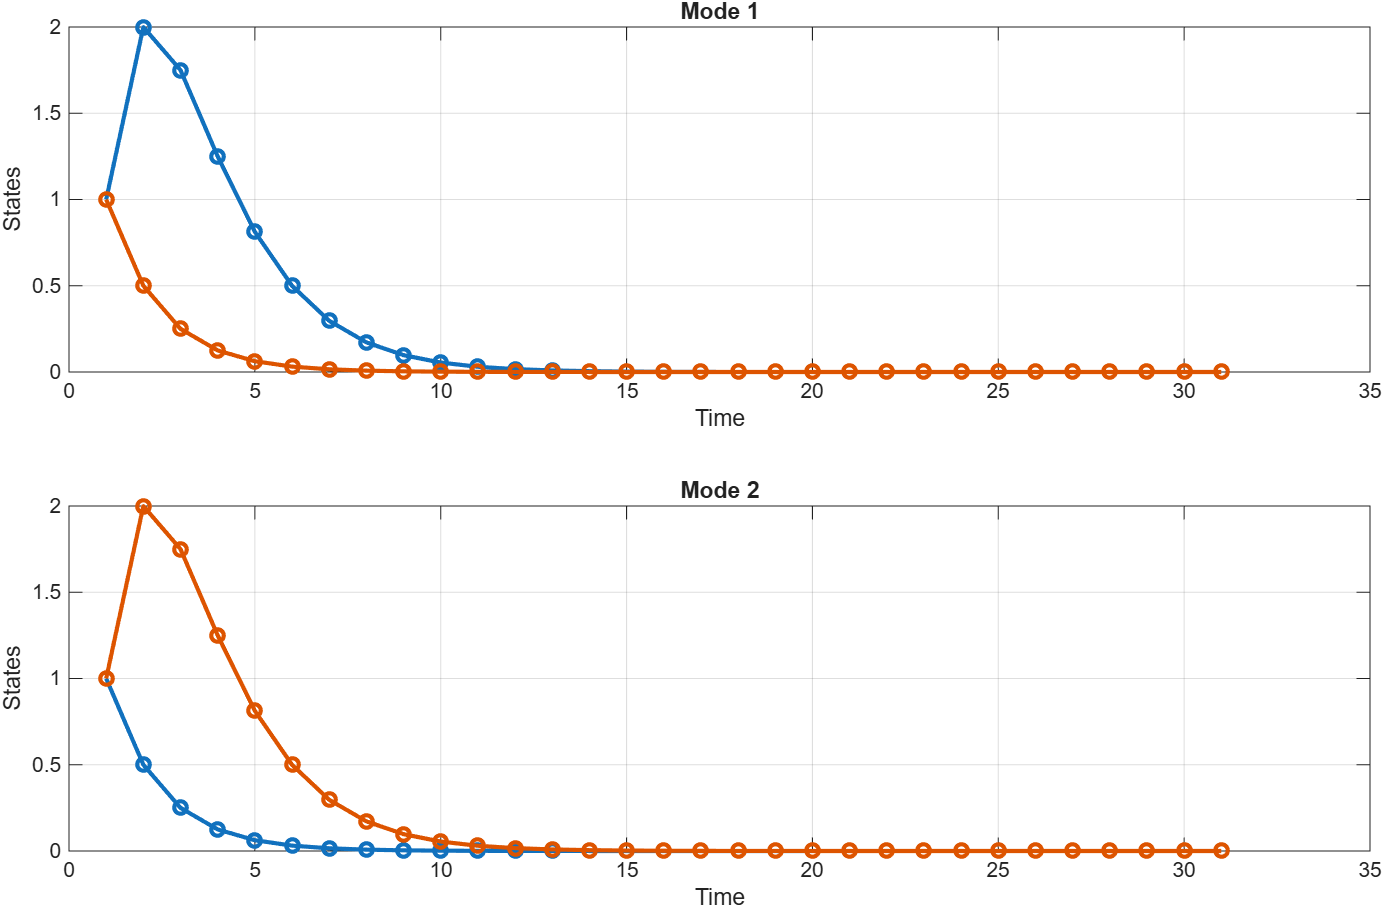
\includegraphics[width=\textwidth]{mjls_example1.png}
        \caption{Stable trajectories when the system operates in a single mode without switching.}
        \label{fig:mjls_no_switching}
    \end{minipage}
    \hfill
    \begin{minipage}{0.48\textwidth}
        \centering
        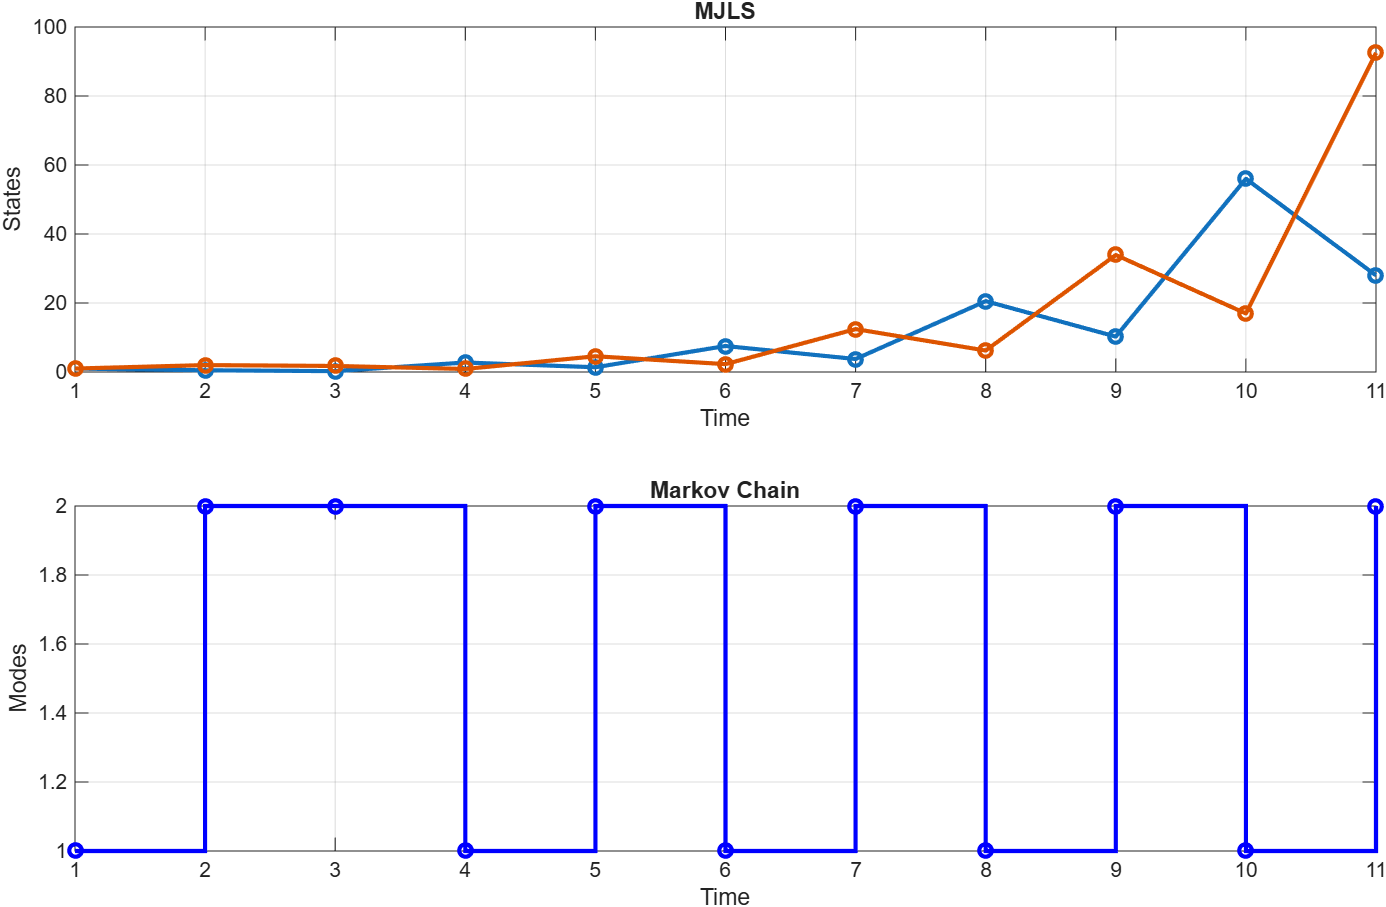
\includegraphics[width=\textwidth]{mjls_instability.png}
        \caption{Unstable, diverging trajectories when switching occurs between two individually stable modes.}
        \label{fig:mjls_switching_instability}
    \end{minipage}
    \caption{Classic counter-intuitive example showing how switching dynamics can cause instability in switched systems.}
    \label{fig:mjls_instability_demo}
\end{figure}


\begin{mytheorem}{Lyapunov MSS Characterization}
The autonomous MJLS $x_{k+1} = A_i x_k$ is Mean Square Stable if and only if there exist $N$ symmetric positive definite matrices $P_1, P_2, \dots, P_N \succ 0$ satisfying the coupled Lyapunov inequalities:
\begin{equation}
    \sum_{j=1}^N p_{ij} A_i^\trp P_j A_i - P_i \prec 0, \quad \forall i \in \mathcal{S} . \label{eq:mjls_coupled_lyap}
\end{equation}
\end{mytheorem}

\begin{proof}
We prove the sufficiency ($\Leftarrow$) of this theorem. Assume there exist positive definite matrices $P_i \succ 0$ satisfying the coupled inequalities \eqref{eq:mjls_coupled_lyap}. We propose a mode-dependent Lyapunov function:
\begin{equation}
V(x_k, \theta_k) = x_k^\trp P(\theta_k) x_k \ge 0, \quad \text{where } P(\theta_k) = P_i \text{ when } \theta_k = i ,
\end{equation}
We analyze the conditional expectation of $V(x_{k+1}, \theta_{k+1})$ given the state $x_k$ and mode $\theta_k = i$:
\begin{equation}
\mathbb{E}\left[ V(x_{k+1}, \theta_{k+1}) \ \middle| \ x_k, \theta_k = i \right] = \mathbb{E}\left[ x_{k+1}^\trp P(\theta_{k+1}) x_{k+1} \ \middle| \ x_k, \theta_k = i \right] ,
\end{equation}
Substituting the state dynamics $x_{k+1} = A_i x_k$:
\begin{align}
    \mathbb{E}\left[ V(x_{k+1}, \theta_{k+1}) \ \middle| \ x_k, \theta_k = i \right] &= \mathbb{E}\left[ x_k^\trp A_i^\trp P(\theta_{k+1}) A_i x_k \ \middle| \ x_k, \theta_k = i \right] \nonumber \\
&= x_k^\trp A_i^\trp \mathbb{E}\left[ P(\theta_{k+1}) \ \middle| \ \theta_k = i \right] A_i x_k ,
\end{align}
The conditional expectation of the matrix $P(\theta_{k+1})$ is the sum of the matrices weighted by the transition probabilities:
\begin{equation}
\mathbb{E}\left[ P(\theta_{k+1}) \ \middle| \ \theta_k = i \right] = \sum_{j=1}^N p_{ij} P_j ,
\end{equation}
Thus, we have:
\begin{equation}
\mathbb{E}\left[ V(x_{k+1}, \theta_{k+1}) \ \middle| \ x_k, \theta_k = i \right] = x_k^\trp \left( A_i^\trp \left( \sum_{j=1}^N p_{ij} P_j \right) A_i \right) x_k ,
\end{equation}
Subtracting $V(x_k, i) = x_k^\trp P_i x_k$ yields the expected variation:
\begin{equation}
\mathbb{E}\left[ V(x_{k+1}, \theta_{k+1}) \ \middle| \ x_k, \theta_k = i \right] - V(x_k, i) = x_k^\trp \left( \sum_{j=1}^N p_{ij} A_i^\trp P_j A_i - P_i \right) x_k ,
\end{equation}
Since the coupled inequalities \eqref{eq:mjls_coupled_lyap} are strictly negative definite, there exists a scalar $\epsilon > 0$ such that:
\begin{equation}
\mathbb{E}\left[ V(x_{k+1}, \theta_{k+1}) \ \middle| \ x_k, \theta_k = i \right] - V(x_k, i) \le -\epsilon \| x_k \|^2 ,
\end{equation}
Taking the total expectation across all possible trajectories:
\begin{equation}
\mathbb{E}\left[ V(x_{k+1}, \theta_{k+1}) \right] - \mathbb{E}\left[ V(x_k, \theta_k) \right] \le -\epsilon \mathbb{E}\left[ \| x_k \|^2 \right] ,
\end{equation}
Summing this inequality from $k = 0$ to $M$:
\begin{equation}
\mathbb{E}\left[ V(x_{M+1}, \theta_{M+1}) \right] - \mathbb{E}\left[ V(x_0, \theta_0) \right] \le -\epsilon \sum_{k=0}^M \mathbb{E}\left[ \| x_k \|^2 \right] ,
\end{equation}
Rearranging and noting that $V(x, \theta) \ge 0$:
\begin{equation}
\sum_{k=0}^M \mathbb{E}\left[ \| x_k \|^2 \right] \le \frac{1}{\epsilon} \mathbb{E}\left[ V(x_0, \theta_0) \right] ,
\end{equation}
Taking the limit as $M \to \infty$, the infinite sum is bounded, which implies:
\begin{equation}
\lim_{k \to \infty} \mathbb{E}\left[ \| x_k \|^2 \right] = 0 ,
\end{equation}
This establishes Mean Square Stability.
\end{proof}

\section{Optimal Control of MJLS (MJLS-LQR)}
We now design an optimal state feedback controller for the system \eqref{eq:mjls_system} to minimize the infinite-horizon quadratic cost function:
\begin{equation}
J = \mathbb{E}\left[ \sum_{k=0}^\infty \left( x_k^\trp Q(\theta_k) x_k + u_k^\trp R(\theta_k) u_k \right) \right] ,
\end{equation}
where $Q(i) = Q_i \ge 0$ and $R(i) = R_i \succ 0$ are the state and control weighting matrices for each mode $i \in \mathcal{S}$.

Because the plant dynamics switch, the optimal controller must be mode-dependent:
\begin{equation}
u_k^* = -K_i x_k \quad \text{when } \theta_k = i ,
\end{equation}
Using dynamic programming, the mode-dependent feedback gains $K_i$ and the optimal cost-to-go matrices $P_i$ are found by solving the \textbf{Coupled Discrete Algebraic Riccati Equations (CDARE)}.

\begin{mytheorem}{Optimal MJLS-LQR Controller}
If the MJLS is stabilizable and detectable in the mean square sense, then:
\begin{enumerate}
    \item The Coupled Discrete Algebraic Riccati Equations:
    \begin{equation}
        P_i = A_i^\trp \mathcal{E}_i(P) A_i - A_i^\trp \mathcal{E}_i(P) B_i \left( R_i + B_i^\trp \mathcal{E}_i(P) B_i \right)^{-1} B_i^\trp \mathcal{E}_i(P) A_i + Q_i , \label{eq:mjls_cdare}
    \end{equation}
    where:
    \begin{equation}
        \mathcal{E}_i(P) = \sum_{j=1}^N p_{ij} P_j , \label{eq:mjls_operator}
    \end{equation}
    possess unique symmetric positive definite solutions $P_1, P_2, \dots, P_N \succ 0$.
    \item The optimal state feedback gain for mode $i \in \mathcal{S}$ is:
    \begin{equation}
        K_i = \left( R_i + B_i^\trp \mathcal{E}_i(P) B_i \right)^{-1} B_i^\trp \mathcal{E}_i(P) A_i , \label{eq:mjls_opt_k}
    \end{equation}
    \item The resulting closed-loop system is Mean Square Stable.
\end{enumerate}
\end{mytheorem}
The operator $\mathcal{E}_i(P)$ couples the Riccati equations: to solve for $P_i$ in one mode, we must know the solution $P_j$ in all other reachable modes. This is a fundamental difference from independent mode-by-mode design and ensures that the controller accounts for future switching.

\section{Application: Networked Control Systems (NCS)}
A critical application of MJLS is the modeling and control of \textbf{Networked Control Systems (NCS)}. In an NCS, the control loop is closed through a digital communication network. Transmission delays and packet dropouts occur randomly due to network traffic congestion and wireless interference.

\begin{figure}[H]
    \centering
    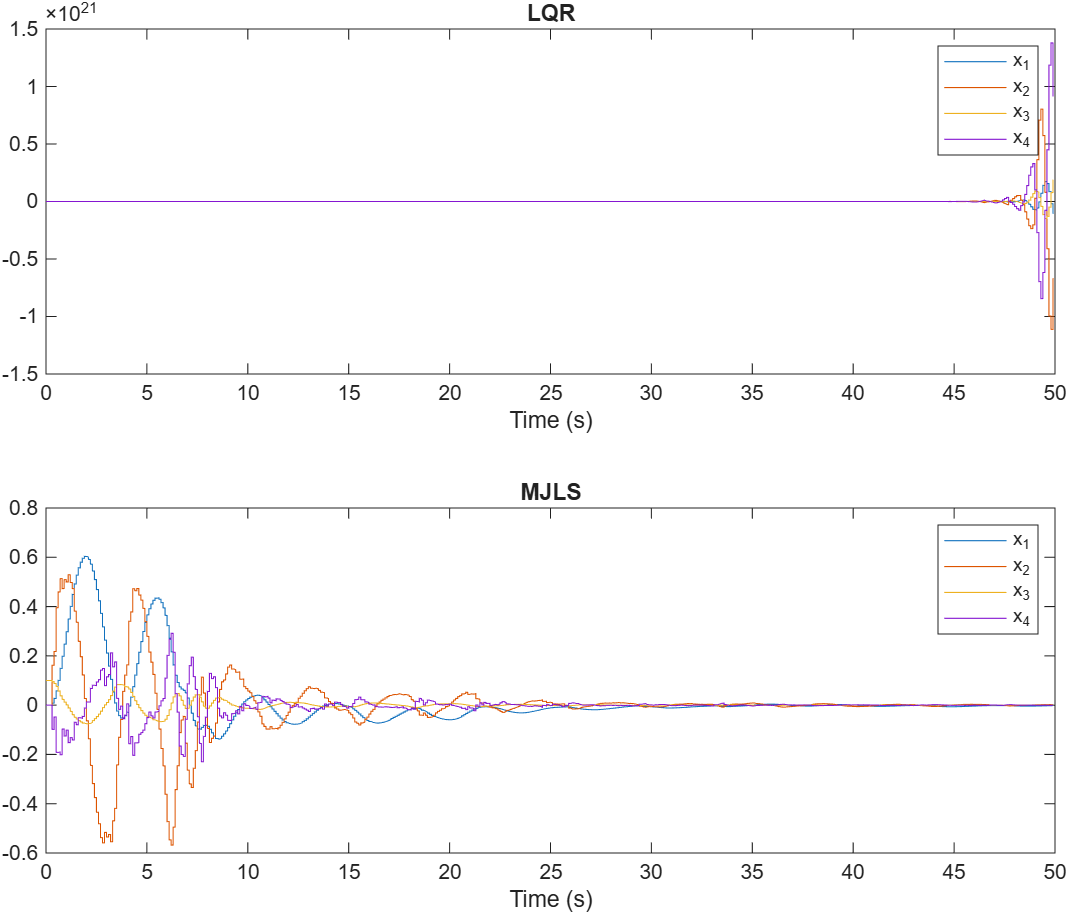
\includegraphics[width=10cm]{mjls_ncs_pendulo.png}
    \caption{A Networked Control System setup: controlling an inverted pendulum where the control signal is transmitted over a lossy communication network subject to random packet dropouts.}
    \label{fig:mjls_ncs}
\end{figure}

As shown in Figure~\ref{fig:mjls_ncs}, we model the lossy channel as a Markov chain with two modes $\theta_k \in \{1, 2\}$:
- \textbf{Mode 1 (Transmission Success)}: The packet is transmitted successfully. The controller updates the input: $u_k = -K x_k$. The dynamics are governed by the closed-loop matrix $A_1 = A - BK$.
- \textbf{Mode 2 (Transmission Failure)}: The packet is dropped. The ZOH holds the previous control signal constant: $u_k = u_{k-1}$. The system is unforced or operates under a delayed feedback loop, yielding $A_2 = A$.

The switching between these modes is governed by a Markov chain, where the transition probabilities represent the reliability of the communication channel.

\begin{figure}[H]
    \centering
    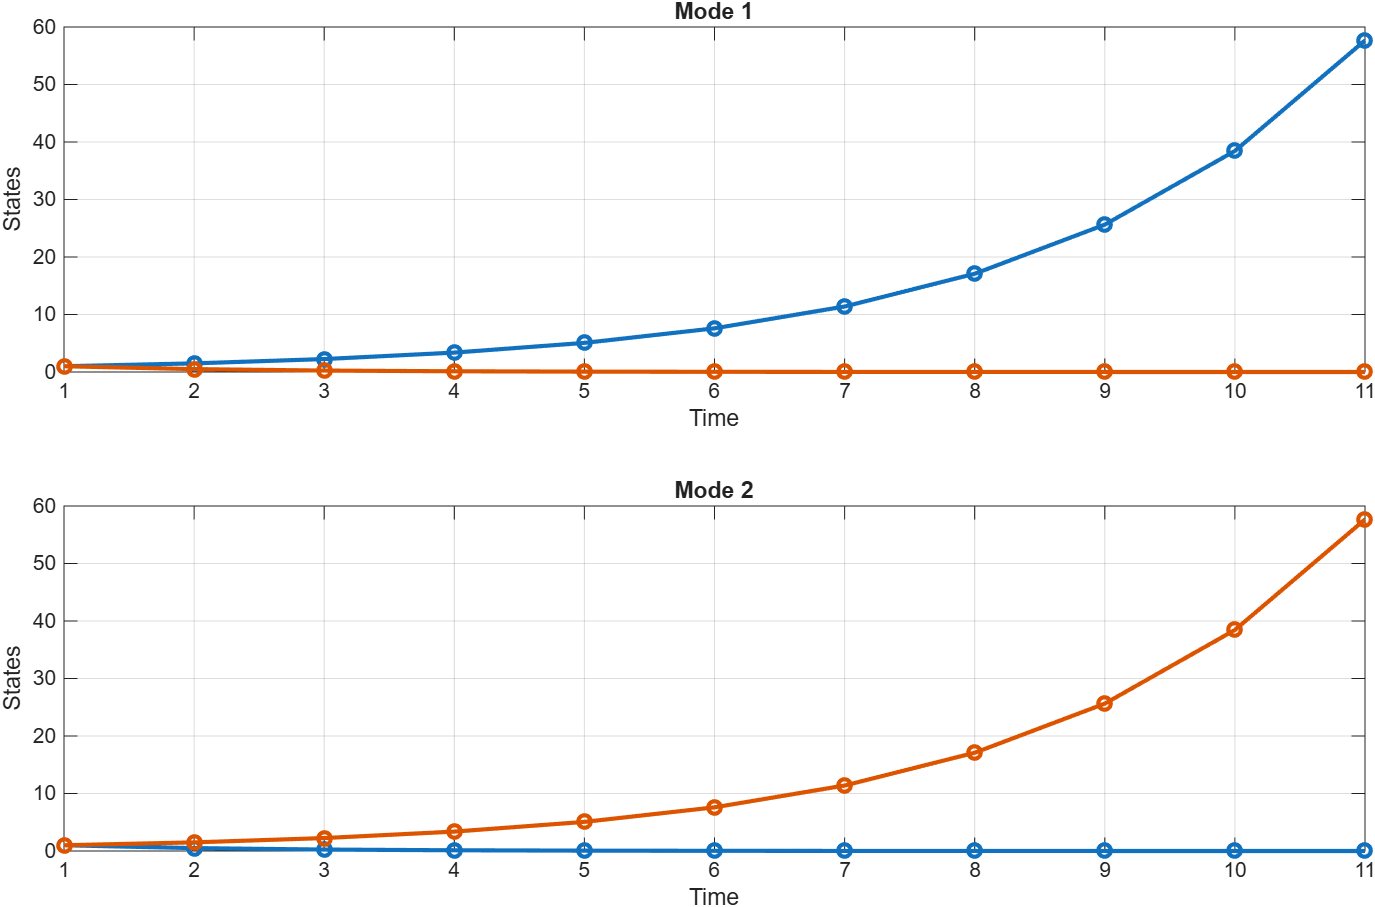
\includegraphics[width=9cm]{mjls_example2.png}
    \caption{Simulated state trajectories $x_1(k)$ and $x_2(k)$ of a Mean Square Stable MJLS under Markovian switching, showing convergence to the origin despite constant mode changes.}
    \label{fig:mjls_traj}
\end{figure}

\begin{figure}[H]
    \centering
    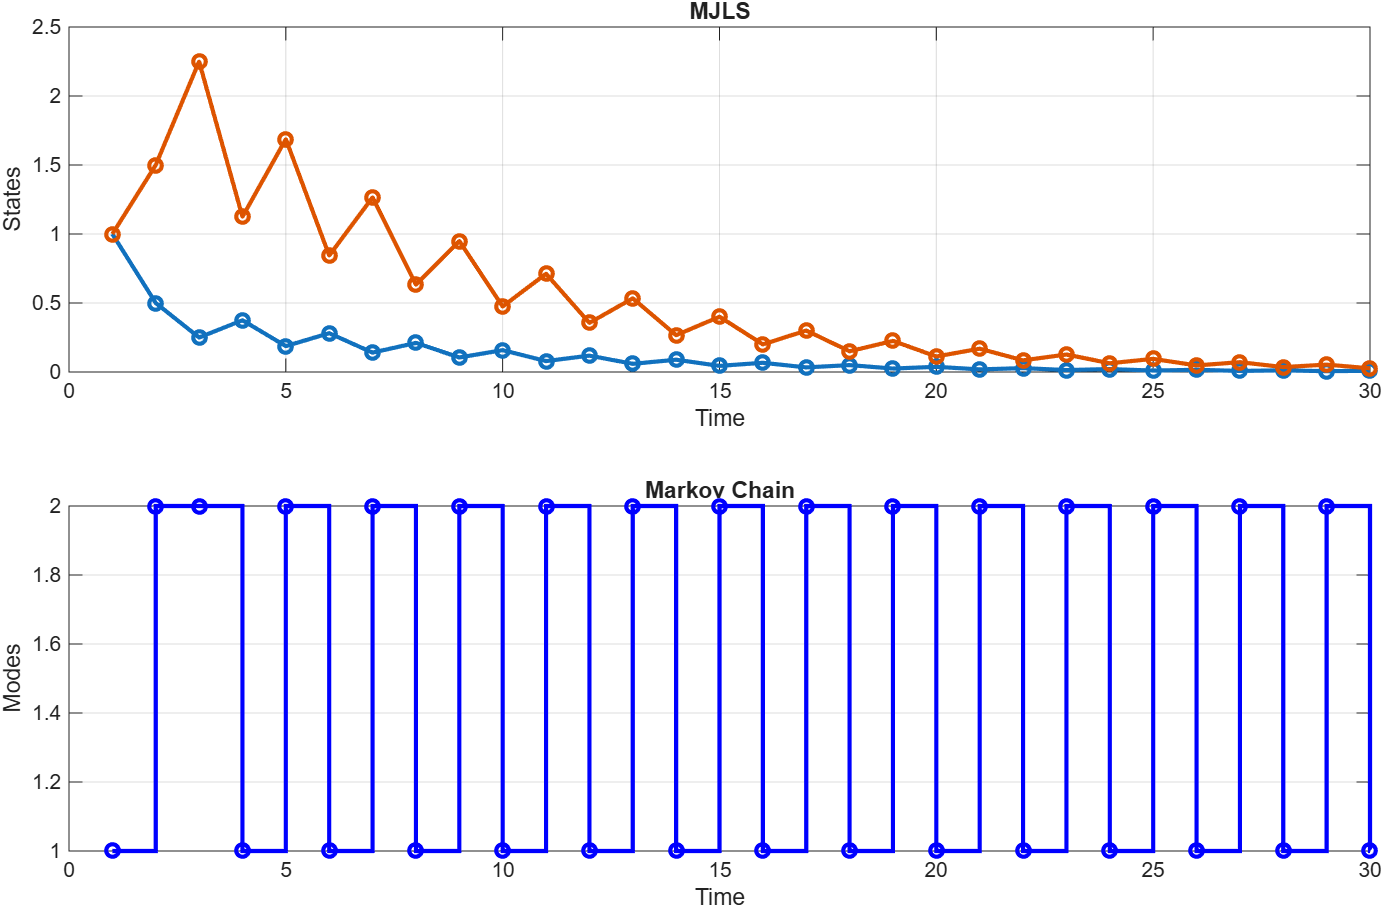
\includegraphics[width=9cm]{mjls_example2_switching.png}
    \caption{The active operating mode $\theta_k \in \{1, 2, 3, 4\}$ of the system during the simulation, showing fast, random switching governed by the transition probability matrix.}
    \label{fig:mjls_switching}
\end{figure}

Figures~\ref{fig:mjls_traj} and \ref{fig:mjls_switching} demonstrate the simulation of a 4-mode MJLS. Although individual modes may be highly oscillatory or unstable on their own, the coupled Markov feedback design guarantees that the joint state trajectory converges asymptotically to the origin in the mean square sense, illustrating the robustness and mathematical elegance of the MJLS framework.


\end{document}
